% !TEX encoding = UTF-8 Unicode
%% LaTeX2e file `clb-template.tex'
%% generated by the `filecontents' environment
%% from source `CLaTeX' on 2012/04/26.
%%
\documentclass{clbthesis}
% insert additional packages here e.g., 
% to use `Umlaute'

%
%=================================================================
 % !TEX encoding = UTF-8 Unicode
% ÄÖÜ ß äöü



\usepackage[utf8]{inputenc}			% Eingabekodierung
\usepackage[ngerman,english]{babel}	% Unterstütze deutsch und englisch, english ist aktiv, \selectlanguage{ngerman}
\usepackage[T1]{fontenc}				% Korrekte Umlaute im PDF

%\usepackage{ucs}
\usepackage{blindtext}				% Blindtext einfach erzeugen
\usepackage{listings}
\usepackage{floatflt}
\usepackage{color}

%\lstset{
%extendedchars=\true,
%inputencoding=utf8x
%}

\lstset{
extendedchars=\true,
language=XML,                             % Code langugage
basicstyle=\ttfamily,                   % Code font, Examples: \footnotesize, \ttfamily
%keywordstyle=\color{OliveGreen},        % Keywords font ('*' = uppercase)
keywordstyle=\color{blue},        % Keywords font ('*' = uppercase)
commentstyle=\color{red},              % Comments font
numbers=left,                           % Line nums position
numberstyle=\tiny,                      % Line-numbers fonts
stepnumber=1,                           % Step between two line-numbers
numbersep=5pt,                          % How far are line-numbers from code
%backgroundcolor=\color{lightlightgray}, % Choose background color
frame=none,                             % A frame around the code
tabsize=2,                              % Default tab size
captionpos=b,                           % Caption-position = bottom
breaklines=true,                        % Automatic line breaking?
breakatwhitespace=false,                % Automatic breaks only at whitespace?
showspaces=false,                       % Dont make spaces visible
showtabs=false,                         % Dont make tabls visible
columns=flexible,                       % Column format
morekeywords={__global__, __device__,array,dict,string,integer,key},  % CUDA specific keywords
}

\usepackage{varioref}
\newcommand{\figref}[1]{(figure \vref{#1})}
\newcommand{\tabref}[1]{(table \vref{#1})}
\newcommand{\seeref}[1]{(see \vref{#1})}
\newcommand{\reff}[1]{„\nameref{#1}“ (see \vref{#1})}
\newcommand{\USD}[1]{{#1}\,\$}

% ############################################################################
% Metadaten und anklickbare Verweise in der PDF-Datei
% ===========================================
%\usepackage[pdftex
%	, pdfauthor={Alexander Maringele}
%	, pdftitle={An Interactive Interface for BoolTool}
%	, pdfsubject={bachaelor thesis},
%		%,pdfkeywords={}
%		%,pdfproducer={Latex with hyperref}
%		%,pdfcreator={pdflatex}
%	, colorlinks=true
%]
%{hyperref}				% anklickbare Links im PDF

% \usepackage[pdftex]{hyperref}

% to typeset algorithms
% \usepackage{algorithm}
% \usepackage{algorithmic}
% for documentation of packages search
% http://ctan.org

\pdfinfo{
/Author (Alexander Maringele)
/Title  (Interactive Interface for Bool Tool)
/CreationDate (D:20121001121300)
/Subject (iPad Learning App for Propositional Logic)
/Keywords (University of Innsbruck;Institute of Computer Science;Computational Logic)
}
% ##############################################################################

\usepackage{graphicx}  % \includgraphics
\usepackage{amssymb}

\usepackage[xindy,toc,nonumberlist]{glossaries}
 % !TEX encoding = UTF-8 Unicode

\newglossaryentry{computer}
{
  name=computer,
  description={is a programmable machine that receives input,
               stores and manipulates data, and provides
               output in a useful format}
}

\newglossaryentry{naiive}
{
  name=na\"{\i}ve,
  description={is a French loanword (adjective, form of naïf)
               indicating having or showing a lack of experience,
               understanding or sophistication}
}


 \makeglossaries


% #########################################################
% smarter line breaks for urls
% =========================================================
%\let\oldurlbreaks=\UrlBreaks
%\renewcommand{\UrlBreaks}{\oldurlbreaks\do\a\do\b\do\c\do\d\do\e%
%  \do\f\do\g\do\h\do\i\do\j\do\k\do\l\do\m\do\n\do\o\do\p\do\q%
%  \do\r\do\s\do\t\do\u\do\v\do\w\do\x\do\y\do\z\do\?\do\&}
%\renewcommand{\UrlBreaks}{\oldurlbreaks\do\-\do\&}
% #########################################################

 
%=================================================================

\begin{document}
%__________________________________________
%---- show all bibliography entries
% \nocite{*}
%–––––––––––––––––––––––––––––––––––––––––

% BEGIN: titlepage setup -------------------------------------------
\title{\Nyaya for iPad\vspace{0.5cm}\\ \LARGE{Interactive Environment for BoolTool}}
\mailaddress{alexander.maringele@gmail.com}
\matriculationnumber{8517725}
\author{Alexander~Maringele}
\date{
\includegraphics[width=6cm]{pics/NyayaAppIcon1024.png}\\ \today}
\supervisor{Dr.~Georg~Moser}


% END: titlepage setup ----------------------------------------------
\maketitle

\abstract{% !TEX encoding = UTF-8 Unicode

%% LaTeX2e file `abstract.tex'
%% generated by the `filecontents' environment
%% from source `CLaTeX' on 2012/04/26.
%%


\begin{minipage}[t]{180mm}
\begin{verse}
If wishes were horses \\
Beggars would ride: \\
If turnips were watches \\
I would wear one by my side. \\
And if if's and an's were pots and pans, \\
The tinker would never work!
\end{verse}.
\end{minipage}

This nursery rhyme from the 16th century has some propositions! But are they true? 
Propositional logic provides a toolset to answer this question and many other questions,
where propositions are made and connected. 
\Nyaya for iPad
will introduce the formalism of propositional logic interactively.
A series of tutorials will put the user in a position
to formalize this poem
and to asses if the implications made by this poem can be true.
%\vspace{1cm}\\
%\begin{minipage}[b]{180mm}
%\begin {verse}
%Hello
%\end{verse}
%\end{minipage}}

\acknowledgments{I am grateful to my family for their support and encouragement. \\ \\
I thank my employer World-Direct eBussiness Solutions GmbH for its understanding of certain absences. \\ \\
Last but not least I want to thank Dr.\ Georg Moser for accepting and supervising the project.}

\tableofcontents
%====================================================================
% BEGIN: CONTENT ----------------------------------------------------
%====================================================================
\chapter{Introduction} 			
% 1 pages
% !TEX encoding = UTF-8 Unicode

\begin{quote}
\em The aim of logic in computer science is to develop languages 
to model the situations we encounter as computer science professionals, 
in such way that we can reason about them formally. \cite{Huth:2004:LCS:975331}
\end{quote}

Logic is used daily. Although the core of reasoning and the foundation of computer science, 
logic still takes time and practice to be mastered soundly and completely. 
Uncertainty in the formalisms of logic leads to fundamental inaccuracies 
in the modeling of various applications in computer science. 
Therefore logic is a mandatory part of every computer science curriculum. 

Each tool that promotes a deeper and more accurate understanding of formalisms and applications of logic,
or simply provides an easier introduction to formal logic, 
is a welcome addition to the toolbox of training.


\paragraph{Propositional logic}is – to put it simply - the entry point and the innermost core of logic. 
It is a powerful formal language, which can be used in many fields. 
But it also has limits of expressiveness and so 
there are many more powerful formal languages of logic, 
which can not be mastered without a sufficient understanding  of propositional logic.

\paragraph{BoolTool}by the Computational Logic Research Group at the University of Innsbruck allows the manipulation and evaluation of Boolean functions. The tool supports different representations of Boolean functions and a variety of different algorithms.
Propositional logic is one of many representations of Boolean functions.

\paragraph{\Nyaya}“{\em (sanskrit ny-$\bar{\mbox{a}}$yá, literally 'recursion’  used in the sense of  ‘syllogism, inference’) is [...] one of the [...] schools of Hindu philosophy – specifically the school of logic.}”\ \cite{WIKIPEDIA:NYAYA}
%\footnote{\href{http://en.wikipedia.org/wiki/Nyaya}{ en.wikipedia.org/wiki/Nyaya}}. 
“{\em Its followers believed that obtaining valid knowledge was the only way  to obtain release from suffering.}”\ \cite{IEP:NYAYA} 
%\footnote{\href{http://www.iep.utm.edu/nyaya/}{ www.iep.utm.edu/nyaya/}}

\paragraph{\Nyaya for iPad}provides an interactive environment,
that allows the user to learn simple facts about the formalism of propositional logic 
and standard transformations of Boolean functions. 
The environment is self-explanatory, re-implements the functionality of  BoolTool,
provides a graphical editor for syntax trees of propositional formulas, and 
works without a back end on a server.
\Nyaya supports the most effective learning techniques – 
steadily learning and practice testing\ \cite{Dunlosky01012013} –
with its combination 
of small bits of learning content and seemingly countless exercises. 


%\section{Why iPad?}
%
%It‘s popular, it‘s available and has a one defined form factor.


\chapter{Related Work}						
% 2 pages (complete)
% !TEX encoding = UTF-8 Unicode

Of course, Ny$\bar{a}$ya for iPad is not the first program,  that processes expressions of propositional logic. 
Besides powerful SAT-solvers and automatic provers, which rarely can be used by beginners,
there are some applications, than can be used on a basic level.  
Most of them provide a (short) introduction to propositional logic, but they seldom offer tutorials or exercises. 	

The following overview focuses on applications accessible
per website and apps available for iPad.

\section{Websites}

\begin{itemize}
\item 
\href{http://www.cs.wfu.edu/~burg/JavaPackages/indexswingnet.html}{\bf PLogic Applet} 
by S. Lukins, A. Levicki, and 
\href{http://www.cs.wfu.edu/~burg}{J. Burg} at the
\href{http://www.cs.wfu.edu}{Wake Forest University}, is a
tutorial program for propositional logic 
“that serves a double role as an educational tool and a research environment”\footnote {
\url{http://www.cs.wfu.edu/~burg/papers/PropLogic.pdf}} and focuses 
 on interactive theorem-proving.

\item
\href{http://cl-informatik.uibk.ac.at/software/booltool/}{\bf 

\includegraphics[width=0.8cm]{clshortlogo_new.pdf}BoolTool} 
by the 
\href{http://cl-informatik.uibk.ac.at/}{Computational Logic} 
research group at the 
\href{http://informatik.uibk.ac.at}{University of Innsbruck}
“is an interface to the program BoolTool which allows the manipulation and evaluation of boolean functions.”\footnote{
\url{http://cl-informatik.uibk.ac.at/software/booltool/?page=info}}. 
It computes truth tables and binary decision diagrams and checks for satisfiability and validity.

\end{itemize}

\section{Apps for iPad}
 
Some apps for iPad or iPod touch handle aspects of propositional logic.

\begin{itemize}

\item  \href{http://itunes.apple.com/at/app/constraints/id418722652?mt=8}{\bf 

\includegraphics[width=0.8cm]{AppStore/Constraints.png} Constraints}
by 
\href{http://www.mysvc.it/myapps/constraints/}{Davide Cucciniello} 
is a “SAT based propositional (boolean) logic engine defined by a list of models, 
where a model includes a list of constraints (a Knowledge Base) 
each defined by a propositional formula (x and (y or not z)) 
including a set of propositional (boolean) variables (x,y,z) 
and operators (and,or,not).”\footnote{
\url{http://www.mysvc.it/myapps/constraints/}} 
let's you build models in an interactive way. It also provides a short introduction in propositional logic, but no tutorials.


\item \href{http://itunes.apple.com/at/app/truth-table-generator/id507190346?mt=8}{\bf 
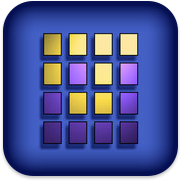
\includegraphics[width=0.8cm]{AppStore/TruthTable.png} Truth Table Generator} 
by
\href{http://www.mertzwerkz.com/truth.html}{Mertz Werkz LLP}    
“constructs truth tables for the Boolean expressions you enter”.\footnote{
\url{http://www.mertzwerkz.com/truth.html}}
It does that nicely by using standard symbols of propositional logic (and a limited set of atoms), but nothing more.

\item
\href{http://itunes.apple.com/at/app/boolean-logic-cheat-sheet/id341959531?mt=8}{\bf 
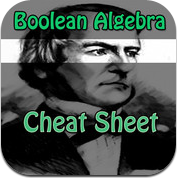
\includegraphics[width=0.8cm]{AppStore/CheatSheet.png} Boolean Logic Cheat Sheet} 
by 
{Clint Johnson} presents two pages of logic “rules and laws“ in low picture quality. So “all of your Boolean 
logic needs.”\footnote{
\url{http://itunes.apple.com/at/app/boolean-logic-cheat-sheet/id341959531?mt=8}} 
does not feel quite right.

\item
\href{http://itunes.apple.com/at/app/logic-mania/id434019152?mt=8}{\bf 

\includegraphics[width=0.8cm]{AppStore/LogicMania.png} Logic Mania} 
by 
{Imagination Creations} presents seven logic gates in a list. 
Their semantics are shown in a per-gate-simulation where the user chooses the input and the app shows the result. 
A combination of gates is not possible. It's quite nice but the statement “THE [sic] reference application for students 
studying logic gates.”\footnote{
\url{http://itunes.apple.com/at/app/logic-mania/id434019152?mt=8}}
seems exaggerated.

\end{itemize}


\chapter{Concept}	
\label{ch:concept}						
% 13 pages (complete)
% !TEX encoding = UTF-8 Unicode
% ÄÖÜ ß äöü

%The aim of this project was to design an interactive environment on a tablet computer 
%that allows the user to learn simple facts about the formalism of propositional logic 
%and standard transformations of Boolean functions. 
%The environment was meant to be self-explanatory. 

The core of this concept builds on tutorials with exercises 
and a playground where the %learned 
acquired knowledge can be used in different modes. 
A glossary of terms and a formula calculator to check formulas will support the user in her learning.

\section{Tutorials}

\Nyaya for iPad covers syntax and semantics of propositional logic, 
but only some basic rules of equivalences.
It introduces normal forms, truth tables and binary decision diagrams 
as different but equivalent representations of Boolean functions.

The structure of the tutorials and the content of the exercises are heavily based on %the according
related sections of the book  
{\em Logic in Computer Science}  by M.~Huth and M.~Ryan. \cite{Huth:2004:LCS:975331}
Additional content was taken from the lecture {\em Logic}  by {A. Middeldorp}. \cite{Middeldorp:2012:LICS}


\begin{table}[htdp]
\begin{center}
\begin{lstlisting}[mathescape,firstnumber=5]
  <array> 		<!-- root with title and sections -->
    <string>Tutorials</string> 					<!-- title -->
    <array>			<!-- section with section title and tutorials-->
      <string>Introduction</string> 				<!-- section title -->
      <array>		<!-- tutorial with title and id -->
        <string>Motivation</string> 	<!-- tutorial title -->
        <string>11</string> 						<!-- tutorial id -->
      </array>
		$\square$
\end{lstlisting}
\caption{Tutorials.plist – the configuration file for all tutorials}
\label{tab:TUTORIALPLIST}
\end{center}
\end{table}%

General and specific configurations for the tutorials and additional content for the exercises 
are stored in simple property lists (see \tabref{tab:PLISTDTD}) %\footnote{
%\href{http://www.apple.com/DTDs/PropertyList-1.0.dtd}{http://www.apple.com/DTDs/PropertyList-1.0.dtd}
%(see \tabref{tab:PLISTDTD}). }, 
which are xml-files with some basic data types for data and collections, 
that can be easily read and interpreted by different programs.
The file “Tutorials.plist” (see \tabref{tab:TUTORIALPLIST}) 
provides the basic data about available tutorial sections and tutorial titles 
to build a navigation menu programmatically.

Every tutorial includes a teaching part with examples (HTML-files in UTF-8 encoding) 
and an interactive knowledge checker with exercises, 
where the user gets immediate feedback. 
Every interactive part will present some instructions to master the task.

\subsection{Introduction}

The first tutorial section with four tutorials gives an informal introduction to modeling, 
i.e.\ the translation from sentences in natural language to sentences in the formal language of propositional logic.
Three of the four tutorials
% \hyperref[tut:11]{\textnumero 11}, 
% \hyperref[tut:12]{\textnumero 12}, and
% \hyperref[tut:13]{\textnumero 13} 
use the same content file to present some questions
to check the user's comprehension. 
The fourth tutorial does not include an exercise.

\begin{table}[htdp]
\begin{center}
\begin{lstlisting}[firstnumber=5]
<array>
  <array> 
    <string>If the barometer falls, then it will rain.</string>
    <string>if p then q</string>
    <string>the barometer falls; it will rain</string>
    <string>p $\rightarrow$ q</string>
  </array>
$\square$
\end{lstlisting}
\caption{QA1.plist – content file for the first three tutorials with exercises}
\label{tab:QA1PLIST}
\end{center}
\end{table}%

The content file “QA1.plist” (see \tabref{tab:QA1PLIST}) contains
an array (starts at line 5) 
of arrays of strings that represents sentences and sample solutions for the 
first three exercises.
The first sentence/solutions array of strings starts at line 7 and ends at line 10. 
The first string in the first array (at line 7) is a sentence, 
which must be analyzed in all three exercises. 
The next string (at line 8) is a correct solution for the first exercise,
the third string (at line 9) is a correct solution for the second exercise,
and the last string in the array (at line 10) is a correct solution for the third exercise.  
The next array of strings would start at line 13.

\begin{table}[htdp]
\begin{center}
\begin{lstlisting}[firstnumber=5]
<dict>
  <key>questionLabelText</key>
  <string>Guess the structure …</string>
  <key>answerLabelText</key>
  <string>Use … </string>
   <key>solutionLabelText</key>
   <string>Sample solution</string>
   <key>questionsFile</key>
   <string>QA1</string>
   <key>solutionIndex</key>
   <integer>1</integer>
</dict>
\end{lstlisting}
\caption{11.plist – configuration file for the first exercise}
\label{tab:11PLIST}
\end{center}
\end{table}

Each tutorial has its own configuration file 
(see \tabref{tab:11PLIST})
with a dictionary that
describes the exercise and defines the index of the sample solution,
with which the user's answer will be checked with some tolerance.
The \verb+solutionIndex+ expresses which string 
is to be used as sample solution in exercise.

\paragraph{Applications – \textnumero 11.}
\label{tut:11}
{\em{}“The aim of logic in general is to reason about situations.”}\ \cite{Huth:2004:LCS:975331} 
The first tutorial shows, how two different paragraphs in natural language 
can be reduced to the same formal sentence {\em“If p and not q, then r. Not r. p. Therefore, q“}. 
If the reasoning is correct, the user can use it in both situations. 

In the interactive part the user has to ‘guess’ the formal structure of composite sentences in natural language. 
The sentence 
\verb+‘If the barometer falls,+ \verb+then it will rain’+ 
from line 7 of \verb+QA1.plist+ (see \tabref{tab:QA1PLIST})
has to be translated into
\verb+‘if p then q’+ from line 8 (the solution index is defined as 1 in \verb+11.plist+, see \tabref{tab:11PLIST}).

\paragraph{Propositions – \textnumero 12.}
\label{tut:12}

The concept of propositions – simple declarative sentences – 
as indivisible building blocks of propositional logic 
is explained in more detail. Some counter-examples are presented 
and the ambiguity of natural language is demonstrated.

The user has to find the propositions in composite sentences. 
The correct answer for 
\verb+‘If the barometer falls,+ \verb+then it will rain’+ 
would be  
\verb+‘the barometer falls; it will rain’+ 
from line 9 
(the solution index is defined as 2 in \verb+12.plist+).


\paragraph{Connectives – \textnumero 13.}
\label{tut:13}
The basic symbols of propositional logic to connect propositions are introduced. 
The symbols “$\rightarrow$”, “$\neg$”, “$\wedge$”, and “$\vee$”
 will replace “if then”, “not”, “and” and “or”. 

The user hast to find a matching formula in propositional logic.
For the sentence
\verb+‘If the barometer falls,+ \verb+then it will rain’+ 
a correct answer is
\verb+‘p+ $\rightarrow$ \verb+q’+ 
from line 10 
(the solution index is defined as 3 in \verb+13.plist+),
but 
‘$\neg p \vee q$’ would be accepted too.

\paragraph{Limits – \textnumero 14.}
\label{tut:14}
Some examples are given to demonstrate that not every situation can be modeled in propositional logic. 
There is no exercise for this tutorial.

% The user has to ‘guess’ whether sentences in natural language are suitable for propositional logic.

\subsection{Syntax}

After the informal introduction into the atoms and connectives of propositional logic, 
the formal aspects of propositional logic will be introduced to the user.
Again each exercise is configured by a configuration file similar to 
\verb+11.plist+ (see \tabref{tab:11PLIST}),
but without a \verb+questionsFile+ or a \verb+solutionIndex+,
because the content of the syntax exercises will be generated by the app.
The user's solution will be checked without tolerance.

\paragraph{Definition – \textnumero 21.}
\label{tut:21}
The definition of well formed formulas is explained by a strict grammar with mandatory parenthesis.

%\begin{table}[htdp]
\begin{center}
\begin{tabular}{rcccccccccc}
$P$	&$::=$	&$p$ 	
	&|		& $(\neg P)$ 
	&|		&  $(P \wedge P)$ 
	&|		&  $(P \vee P)$ 
	&|		&  $(P \rightarrow P)$ \\
\end{tabular}
%\caption{Grammar with mandatory parentheses}
%\label{tab:BNFGRPA}
\end{center}
%\end{table}

The user has to check whether a formula matches this strict definition of 
a propositional formula.
If the formula is well formed, the user has to write down the name of the root connective, 
i.e\ negation, conjunction, disjunction or implication. 
If the formula is not well formed, the user has to leave the answer field empty.

\paragraph{Conventions – \textnumero 22.}
\label{tut:22}
The conventions of precedences and associativity  of connectives to save parentheses are introduced. 
The user has to rewrite formulas from strict syntax to formulas using conventions and vice versa.

%\begin{table}[htdp]
\begin{center}
\begin{tabular}{rccclp{1cm}rcccl}
$P$		&$::=$ & $D$ &|& $D \rightarrow P$ 	&& $N$		&$::=$ & $T$ &|& $\neg N$ \\
$D$		&$::=$ & $C$ &|& $D \vee C$		&& $T$		&$::=$ & $p$ &|& $(P)$		\\
$C$		&$::=$ & $N$ &|& $C \wedge N$ 		\\
\end{tabular}
%\caption{Grammar with precedence and associativity}
%\label{tab:BNFGRPR}
\end{center}
%\end{table}

%\begin{table}[htdp]
%\begin{center}
%\begin{tabular}{rcl}
%P		&$::=$ & D [ $\rightarrow$ P ]\\
%D		&$::=$ & C \{ $\vee$ C \}\\
%C		&$::=$ & N  \{ $\wedge$ N \} \\
%N		&$::=$ & $\neg$N | p | (P) \\
%\end{tabular}
%\caption{EBNF Grammar (with precedences)}
%\label{tab:BNF}
%\end{center}
%\end{table}

\paragraph{Sub-formulas – \textnumero 23.}
\label{tut:23}
Sub-formulas (starting from atoms) are used to build bigger formulas. Big formulas are build from many sub-formulas.
In the exercise the user has to extract the set of sub-formulas from composite formulas. 
A correct answer for 
‘$a \vee b \wedge c$’ would be
‘$a,b,c,b\wedge c, a \vee b \wedge c$‘. 
The order of the sub-formulas does not matter and the user can use parentheses as she likes it.
But no sub-formula may occur more than once. 
So the answer ‘$c, b\wedge c, b, a \vee b \wedge c, a$‘ would be right too, 
but ‘$a,b,c,b\wedge c, b, a \vee b \wedge c$‘ would be a wrong answer.

\paragraph{Syntax Trees – \textnumero 24.}
\label{tut:24}
Syntax trees  are introduced as graphical representations of well formed formulas. 
The user has to write formulas for presented syntax trees. 
The user can use parentheses as she likes, but still the written formulas have to match the syntax trees exactly. 
The formula ‘$a \vee b$’ does not match the syntax tree representing the formula ‘$b \vee a$’, 
where the atom node ‘$a$’ is on the right branch of the disjunction node ‘$\vee$’.

\paragraph{Top and Bottom – \textnumero 25.}
\label{tut:25}
The symbols “$\top$” (top) and “$ \bot$” (bottom) are defined
as abbreviations of conjunctions and disjunctions 
of formulas with their negation). Additional basic equivalences are introduced.
The user has to simplify given formulas using tautologies, contradictions and basic equivalences.
%\begin{table}[htdp]
\begin{center}
\begin{tabular}{cp{0.1cm}c}
$\neg P \vee P \equiv \top \equiv P \vee \neg P$  & &
$\neg P \wedge P \equiv \bot \equiv  P \wedge \neg P$
\end{tabular}
\begin{tabular}{ccc}
$P \vee P \equiv P$ &
$\neg \neg P \equiv P$ & 
$P \wedge P \equiv P$
\end{tabular}
\begin{tabular}{cp{1cm}c}
$P \vee Q \equiv Q \vee P$ & &
$P \wedge Q \equiv Q \wedge P$
\end{tabular}
%\caption{tautologies and contradictions}
%\label{tab:TopBottom}
\end{center}
%\end{table}



%\subsubsection{Simplifying formulas – basic natural deduction rules}
%\label{tut:206}

%(206) The tutorial teaches the simplifying of conjunctions and disjunctions with top, bottom and/or the same sub formulas.
%
%
%
%\begin{table}[htdp]
%\begin{center}
%\begin{tabular}{c|c|c|c|c}
%$\neg \neg P$ & $P \vee P$ & $P \wedge P$ & $P \vee Q$ & $P \wedge Q$\\
%\hline
%$P$ & $P$ & $P$ & $Q \vee P$ & $Q \wedge P$\\
%\end{tabular}
%\caption{basic rules}
%\label{tab:BasicRules}
%\end{center}
%\end{table}
%
%The user has to rewrite some formulas eleminating 
%top, bottom, double negations, conjunctions and disjunctions 
%by using rules from 
%\tabref{tab:TopBottom} and \tabref{tab:BasicRules}.

%\subsubsection{Conjunctive Normal Form} 
%\label{tut:207}
%(207) The syntax of formulas in conjunctive normal form is introduced (\tabref{tab:CNF}) and explained.
%It is shown that some formulas in cnf can be simplified to top.

%
%The user has to guess if a presented formula is in conjunctive normal form
%and if it can be simplified to top ($\top$).


%\subsubsection{Disjunctive Normal Form} 
%\label{tut:208}
%(208) The syntax of formulas in disjunctive normal form is introduced (\tabref{tab:DNF}) and explained.
%It is shown that some formulas in dnf can be simplified to bottom.

%
%The user has to guess if a presented formula is in disjunctive normal form
%and if it can be simplified to bottom ($\bot$).


\subsection{Semantics}

After the introduction of well formed formulas the meaning of logical connectives is defined.
Configuration files are used again, the exercise context is generated randomly by the app, 
but exercise \textnumero 33 
also uses a context file with exemplary entailments that would not be likely generated.

\paragraph{Valuation – \textnumero 31}
\label{tut:31}
The truth assignment for atoms $(p,q,r,…)$ is introduced. 
The extended valuation for negation, conjunction, disjunction and implication is defined.
The valuation of arbitrary formulas by evaluating all sub-formulas is described.
The user has to guess or calculate the evaluation of a given formula with a given truth assignment for the atoms of the formula.

\paragraph{Truth Tables – \textnumero 32}
\label{tut:32}
The concept of truth tables is explained and demonstrated with the basic connectives. 
The valuation of arbitrary formulas by evaluating all sub-formulas is demonstrated again.
The user has to fill in truth tables for formulas with a maximum of three atoms.

\paragraph{Entailment and Equivalence – \textnumero 33}
\label{tut:33}
Semantic entailment and equivalence is defined and explained with various examples.
The user has to guess or calculate whether a given semantic entailment or equivalence holds. 

\paragraph{Satisfiability and Validity – \textnumero 34}
\label{tut:34}
The properties satisfiability and validity of propositional formulas are defined and demonstrated. 
The relationship of these properties with top and bottom is mentioned. 
The user has to guess or calculate whether a given formula is satisfiable or valid.

\subsection{Normal Forms}

The advantages of propositional formulas in special shapes will be emphasized.
%\hyperref[tut:207]{CNFs} and \hyperref[tut:208]{DNFs} are already defined
%in \tabref{tab:CNF} and \tabref{tab:DNF}.
The definitions of implication free forms, negation normal form, 
conjunctive normal forms and disjunctive normal forms will be provided. 
A recipe to transform arbitrary propositional formulas into specific normal forms will be delivered.
Rules to detect satisfiability or validity from normal forms will be mentioned.

\subsubsection{Implication Free Form – \textnumero 41}
\label{tut:41}
By removing the rule $P ::= D \rightarrow P$ in \vref{tut:22} 
and optimizing the resulting grammar
the implication free form is defined for propositional formulas.
The equivalence transformation
for removing implications is presented
and proved with a truth table. 

%\begin{table}[htdp]
\begin{center}
\begin{tabular}{rcccl}
$D$		&$::=$ & $C$ &|& $C \vee D$			\\
$C$		&$::=$ & $N$ &|& $N \wedge C$ 		\\
$N$		&$::=$ & $T$ &|& $\neg N$ 			\\
$T$		&$::=$ & $p$ &|& $(D)$
\end{tabular}
%\caption{Grammar without implications}
%\label{tab:BNFGRIFF}
\end{center}
%\end{table}

The user has to check whether a given formula is implication free.
If the formula is not implication free the user has to transform it into an implication free form
using the equivalence transformation.

\begin{table}[htdp]
\begin{center}
%\begin{tabular}{c}
$P \rightarrow Q \equiv \neg P \;\vee\; Q$
%\end{tabular}
%\caption{Equivalence transformation towards implication free form}
%\label{tab:ET_IFF}
\end{center}
\end{table}

\subsubsection{Negation Normal Form – \textnumero 42}
\label{tut:42}
By removing all rules for arbitrary negations 
and optimizing the resulting grammar, 
the negation normal form is defined  for propositional formulas. 
The equivalence transformations to transform negations of conjunctions,
negations of disjunctions, 
and double negations
into negation normal forms are presented 
and proved with truth tables.

%\begin{table}[htdp]
\begin{center}
\begin{tabular}{rcccl}
$D$		&$::=$ & $C$ 		&|& 	$C \vee D$\\
$C$		&$::=$ & $N$ 		&|& 	$N \wedge C$ \\
$N$		&$::=$ & $(D)$ 	&|& 	$L$\\
$L$		&$::=$ & $p $ 		&|& 	$\neg p$
\end{tabular}
%\caption{Grammar for negation normal form – \textnumero }
%\label{tab:BNFGRNNF}
\end{center}
%\end{table}

The user has to check whether a given formula is in negation normal form.
If the formula is not in negation normal form
the user has to transform it into negation normal form
using the equivalence transformation for implications and the equivalence transformations for negations.
The rule for double negations is already known from \vref{tut:25}.

%\begin{table}[htdp]
\begin{center}
\begin{tabular}{cp{5mm}cp{5mm}c}
$\neg (P \wedge Q) \equiv \neg P \vee \neg Q$& &
$\neg \neg P \equiv P$ & &
$\neg (P \vee Q)  \equiv \neg P \wedge \neg Q$
\end{tabular}
%\caption{Equivalence transformations towards negation normal form}
%\label{tab:ET_NNF}
\end{center}
%\end{table}

\subsubsection{Conjunctive Normal Form – \textnumero 43}
\label{tut:43}
A formula in conjunctive normal form is a conjunctive concatenation of disjunctive clauses.
A disjunctive clause is a disjunctive concatenation of literals. 
A literal is an atom or the negation of an atom. 
The distributions of disjunctions over conjunctions is presented
and proved with a truth table.

%\begin{table}[htdp]
\begin{center}
\begin{tabular}{rcccl}
$C$	&$::=$ & $(D)$ 	&$|$ & $(D) \wedge C$\\
$D$	&$::=$ & $L$ 	&$|$ & $L \vee D$\\
$L$	&$::=$ & $p$ 	&$|$ & $\neg p$ 
\end{tabular}
%\caption{Grammar for conjunctive normal form}
%\label{tab:CNF}
\end{center}
%\end{table}

The user has to rewrite formulas to conjunctive normal forms.  
All presented formulas are in negation normal form 
but may already be in conjunctive normal form.
So at most the user have to apply the distributions of disjunctions over conjunctions 
multiple times
as the equivalence transformations towards conjunctive normal form.

%\begin{table}[htdp]
\begin{center}
\begin{tabular}{cp{5mm}c}
$P \vee (Q \wedge R) \equiv (P\vee Q) \wedge (P\vee R)$ & &
$(P \wedge Q) \vee R \equiv (P\vee R) \wedge (Q\vee R)$
\end{tabular}
%\caption{Equivalence transformations towards conjunctive normal form}
%\label{tab:ET_CNF}
\end{center}
%\end{table}


\subsubsection{Disjunctive Normal Form – \textnumero 44}
\label{tut:44}
A formula in disjunctive normal form is a disjunctive concatenation of conjunctive clauses.
A conjunctive clause is a conjunctive concatenation of literals. 
A literal is an atom or the negation of an atom. 
The distributions of conjunctions over disjunctions is presented
and proved with truth tables.

%\begin{table}[htdp]
\begin{center}
\begin{tabular}{rcccl}
$D$	&$::=$ & $C$ 	&$|$ & $C \;\vee D$\\
$C$	&$::=$ & $L$ 	&$|$ & $L \wedge D$\\
$L$	&$::=$ & $p$ 	&$|$ & $\neg p$
\end{tabular}
%\caption{Grammar for disjunctive normal form}
%\label{tab:DNF}
\end{center}
%\end{table}

The user has to rewrite formulas to disjunctive normal forms. 
All presented formulas are in negation normal form 
but may already be in disjunctive normal form.
So at most the user have to apply the distributions of conjunctions over disjunctions 
multiple times as
equivalence transformations towards disjunctive normal form.


%\begin{table}[htdp]
\begin{center}
\begin{tabular}{cp{5mm}c}
$P \wedge (Q \vee R) \equiv (P\wedge Q) \vee (P\wedge Q)$ 			& &
$(P \wedge Q) \wedge R \equiv (P\wedge R) \vee (Q\wedge R)$
\end{tabular}
%\caption{Equivalence transformations towards disjunctive normal form}
%\label{tab:ET_DNF}
\end{center}
%\end{table}



%\subsubsection{From general formula to CNF or DNF}
%\label{tut:406}
%(406)
%To combination of the previous techniques to reach a equivalent representation in conjunctive or disjunctive normal form is provided.
%The potential exponential growing of the length of these transformations is demonstrated.
%
%The user has to rewrite formulas to a conjunctive or disjunctive normal form.
%The presented formula is in general form
%but may already be in the demanded normal form.
%
%\subsubsection{Validity of CNF}
%\label{tut:407} 
%(407) 
%If every disjunctive clause contains at least two contemplementary literals.
%then a formula in conjunctive normal form  is valid (a tautology).
%
%The user has to guess or calculate satisfiability of formulas in conjunctive normal form.
%
%\subsubsection{Satisfiability of DNF} 
%\label{tut:408}
%(408) 
%If every conjunctive clause contains at least two contemplementary literals,
%then a formula in disjunctive normal form  is not satisfiable (a contradiction).
%
%The user has to to guess or calculate satisfiability of formulas in disjunctive normal form.

\subsection{Binary Decision Diagrams}

The definition of Boolean functions is introduced. 
Propositional formulas and syntax trees from the previous sections are representations of Boolean functions.
Boolean expressions and binary decision diagrams are additional representations of Boolean functions.

\paragraph{Boolean functions - \textnumero 51}
\label{tut:51}
N-ary Boolean functions are introduced as mapping from n-tupels of 0s and 1s to the set ${0,1}$.
The Boolean operators $\bar{ \;\;}\;+\;\cdot\;\oplus$ are introduced as special representations of
specific unitary and binary Boolean functions. 
For convenience  in the exercises
an exclamation mark $!(B)$ 
will be used for the negation of a Boolean expression $B$ instead of the bar $\bar{B}$. 
The user has to guess or calculate the results for composite expressions.

\paragraph{Boolean expressions - \textnumero 52}
\label{tut:52}
The grammar for Boolean expressions is defined. 
The equivalence relation of Boolean expressions is explained.

%\begin{table}[htdp]
\begin{center}
\begin{tabular}{rcccccccccc}
$B$	&$::=$	&$p$ 	
	&|		& $(\overline{B})$ 
	&|		&  $(B \cdot B)$ 
	&|		&  $(B + B)$ 
	&|		&  $(B \oplus B)$ \\
\end{tabular}
%\caption{Grammar for Boolean expressions}
%\label{tab:BNFGRBE}
\end{center}
%\end{table}

The user has to rewrite formulas with propositional symbols into Boolean expressions.
The implication may be a challenge for some users, 
but is doable because the implication free form was introduced 
in an earlier tutorial.

\paragraph{Binary Decisions - \textnumero 53}
\label{tut:53}
Binary decision nodes are introduced. 
The valuation of binary decision trees is explained.
The user has to fill in the result nodes in a binary decision tree for a given Boolean expression.

\paragraph{Binary Decision Diagrams - \textnumero 54}
\label{tut:54}
Arbitrary binary decision diagrams are explained. 
Ordered and reduced binary decision diagrams are introduced.
The user has to check whether a binary decision diagram is ordered and/or reduced.

\section{Playground}

On the playground the user can create arbitrary propositional formulas 
by building syntax trees interactively.
Truth assignments can be applied and will be visualized.
The playground supports a least the following use cases.

\begin{itemize}

\item In the {\em free mode} arbitrary formulas can be created by adding, replacing and removing connectives and atoms. The process starts with an atom, which can be expanded or replaced. 
Connectives can be changed any time, sub-formulas can be reordered.
The smallest possible formula consists of one atom with one symbol from the set $\{ \top, \bot, p, q, r, … \}$.

\item In the {\em locked mode} only equivalence transformations can be applied to nodes (see \tabref{tab:ET:ALL})
– depending on the kind of node. 

\item Truth values can be assigned to leaf nodes, 
which represent the atoms of the corresponding propositional formula. 
By default no truth values are assigned to atoms, which is visualized by a blue color of the node.
A green color represents ‘true’, and a red color ‘false’.
The valuation of connective nodes is calculated automatically 
and displayed using the same blue, green and red colors.

\item Connective nodes of obvious tautologies like
$P \vee \neg P$ or
$P \rightarrow P$ are displayed with a green color – 
independent form the valuation status of any sub-node.

\item Connective nodes of obvious contradictions like $P \wedge \neg P$ are displayed with a red color – 
independent form the valuation status of any sub-node.

\item While working with a syntax tree, the corresponding propositional formula is shown on top of the playground.

\item While selecting a sub-node of the syntax tree – the root of a sub-tree – 
for manipulation the corresponding sub-formula will be highlighted in the corresponding propositional formula.

\end{itemize}


\begin{table}[htdp]
\begin{center}
\begin{tabular}{rcl|rcl}

$P$&$ \TAP{\rightarrow}$&$Q$				&$ $&$\TAP{\neg}$&$\neg P$			\\
\hline
$\neg P $&$ \TAP{\vee}$&$Q$					&$ $&$\TAP{P}$&$ $				\\
\\
$ $&$\TAP{\neg}$&$(P \vee Q)$				&$ $&$ \TAP{\neg}$&$(P \wedge Q)$	\\
\hline
$\neg P$&$\TAP{\wedge}$&$\neg Q$			&$\neg P$&$ \TAP{\vee}$&$\neg Q$	\\
\\
$P$&$\TAP{\vee}$&$P$						&$P$&$ \TAP{\wedge}$&$P$			\\
\hline
$$&$\TAP{P}$&$$							&$$&$ \TAP{P}$&$$					\\
\\
$P$&$\TAP{\vee}$&$\neg P$					&P&$\TAP{\wedge}$&$\neg P$		\\
\hline
$ $&$\TAP{\top}$&$ 	$						&	&$\TAP{\bot}$&$ $				\\
\\
$P$&$\TAP{\vee}$&$\top$					&P	&$\TAP{\wedge}$&$\top$			\\
\hline
$ $&$\TAP{\top}$&$ 	$						&	&$\TAP{P}$&$ $				\\
\\
$P$&$\TAP{\vee}$&$\bot$					&$P$&$ \TAP{\wedge}$&$\bot$		\\
\hline
$ $&$\TAP{P}$&$ $							&$ $&$ \TAP{\bot}$&$ $				\\
\\
$P$&$\TAP{\vee}$&$Q$						&$P$&$ \TAP{\wedge}$&$Q$			\\
\hline
$Q$&$\TAP{\vee}$&$P$						&$Q$&$ \TAP{\wedge}$&$P$			\\
\\
$P$&$\TAP{\vee}$&$(Q\wedge R)$				&$P$&$\TAP{\wedge}$&$(Q\vee R)$			\\
\hline
$(P\vee Q)$&$\TAP{\wedge}$&$(P\vee R)$		&$(P\wedge Q)$&$\TAP{\vee}$&$(P\wedge R)$	\\
\\
$(P\wedge Q)$&$\TAP{\vee}$&$R$				&$(P\vee Q)$&$\TAP{\wedge}$&$R$			\\
\hline
$(P\vee R)$&$\TAP{\wedge}$&$(Q\vee R)$		&$(P\wedge R)$&$\TAP{\vee}$&$(Q\wedge R)$	\\
\\
$P$&$\TAP{\vee}$&$(Q\vee R)$				&$P$&$\TAP{\wedge}$&$(Q\wedge R)$			\\
\hline
$(P\vee Q)$&$\TAP{\vee}$&$R$			&$(P\wedge Q)$&$\TAP{\wedge}$&$R$	\\

\end{tabular}
\caption{Transformations which are offered in locked mode}
\label{tab:ET:ALL}
\end{center}
\end{table}%

\begin{table}[htdp]
\begin{center}
\begin{tabular}{rcl|rcl}

$P$&$ \TAP{\leftrightarrow}$&$Q$					&$P$&$ \TAP{\veebar}$&$Q$			\\
\hline
$P \rightarrow Q $&$ \TAP{\wedge}$&$Q \rightarrow P$	&$\neg(P \rightarrow Q) $&$ \TAP{\vee}$&$\neg (Q \rightarrow P)$				\\

\end{tabular}
\caption{Additional transformations in locked mode}
\label{tab:addnf}
\end{center}
\end{table}%

\section{Glossary}

Terms, definitions and truth tables from the tutorials are listed in the glossary in a searchable and hyperlinked form.

\section{BoolTool}

The interactive environment has to contain the functionality of the
\href{http://cl-informatik.uibk.ac.at/software/booltool/}{BoolTool web frontend}.

\subsection{Input}

In the least the embedded BoolTool must support Latin letters as identifiers for atoms, 
and has to parse the symbols
\verb#T# as top, 
\verb#F# as bottom,
\verb#!# as negation operator, 
\verb#&# as conjunction operator,
\verb#+# as disjunction operator,
\verb#># as implication operator,
\verb#^# as exclusive disjunction operator,
and \verb#(# as left and \verb#)# as right parentheses, 
because these ASCII-symbols can be found on almost every keyboard.

Standard symbols “$ \neg \vee \wedge \rightarrow $” 
and additional symbols of propositional logic and Boolean expressions
should be accepted too (see \tabref{tab:BASICSYMBOLS}) 
to make extended or custom keyboards more useful.
A limitation to Latin characters should be avoided, since, for example, 
Chinese symbols also make good identifiers. (\figref{fig:BoolToolChineseInput}).

\begin{figure}[htbp]
\begin{center}
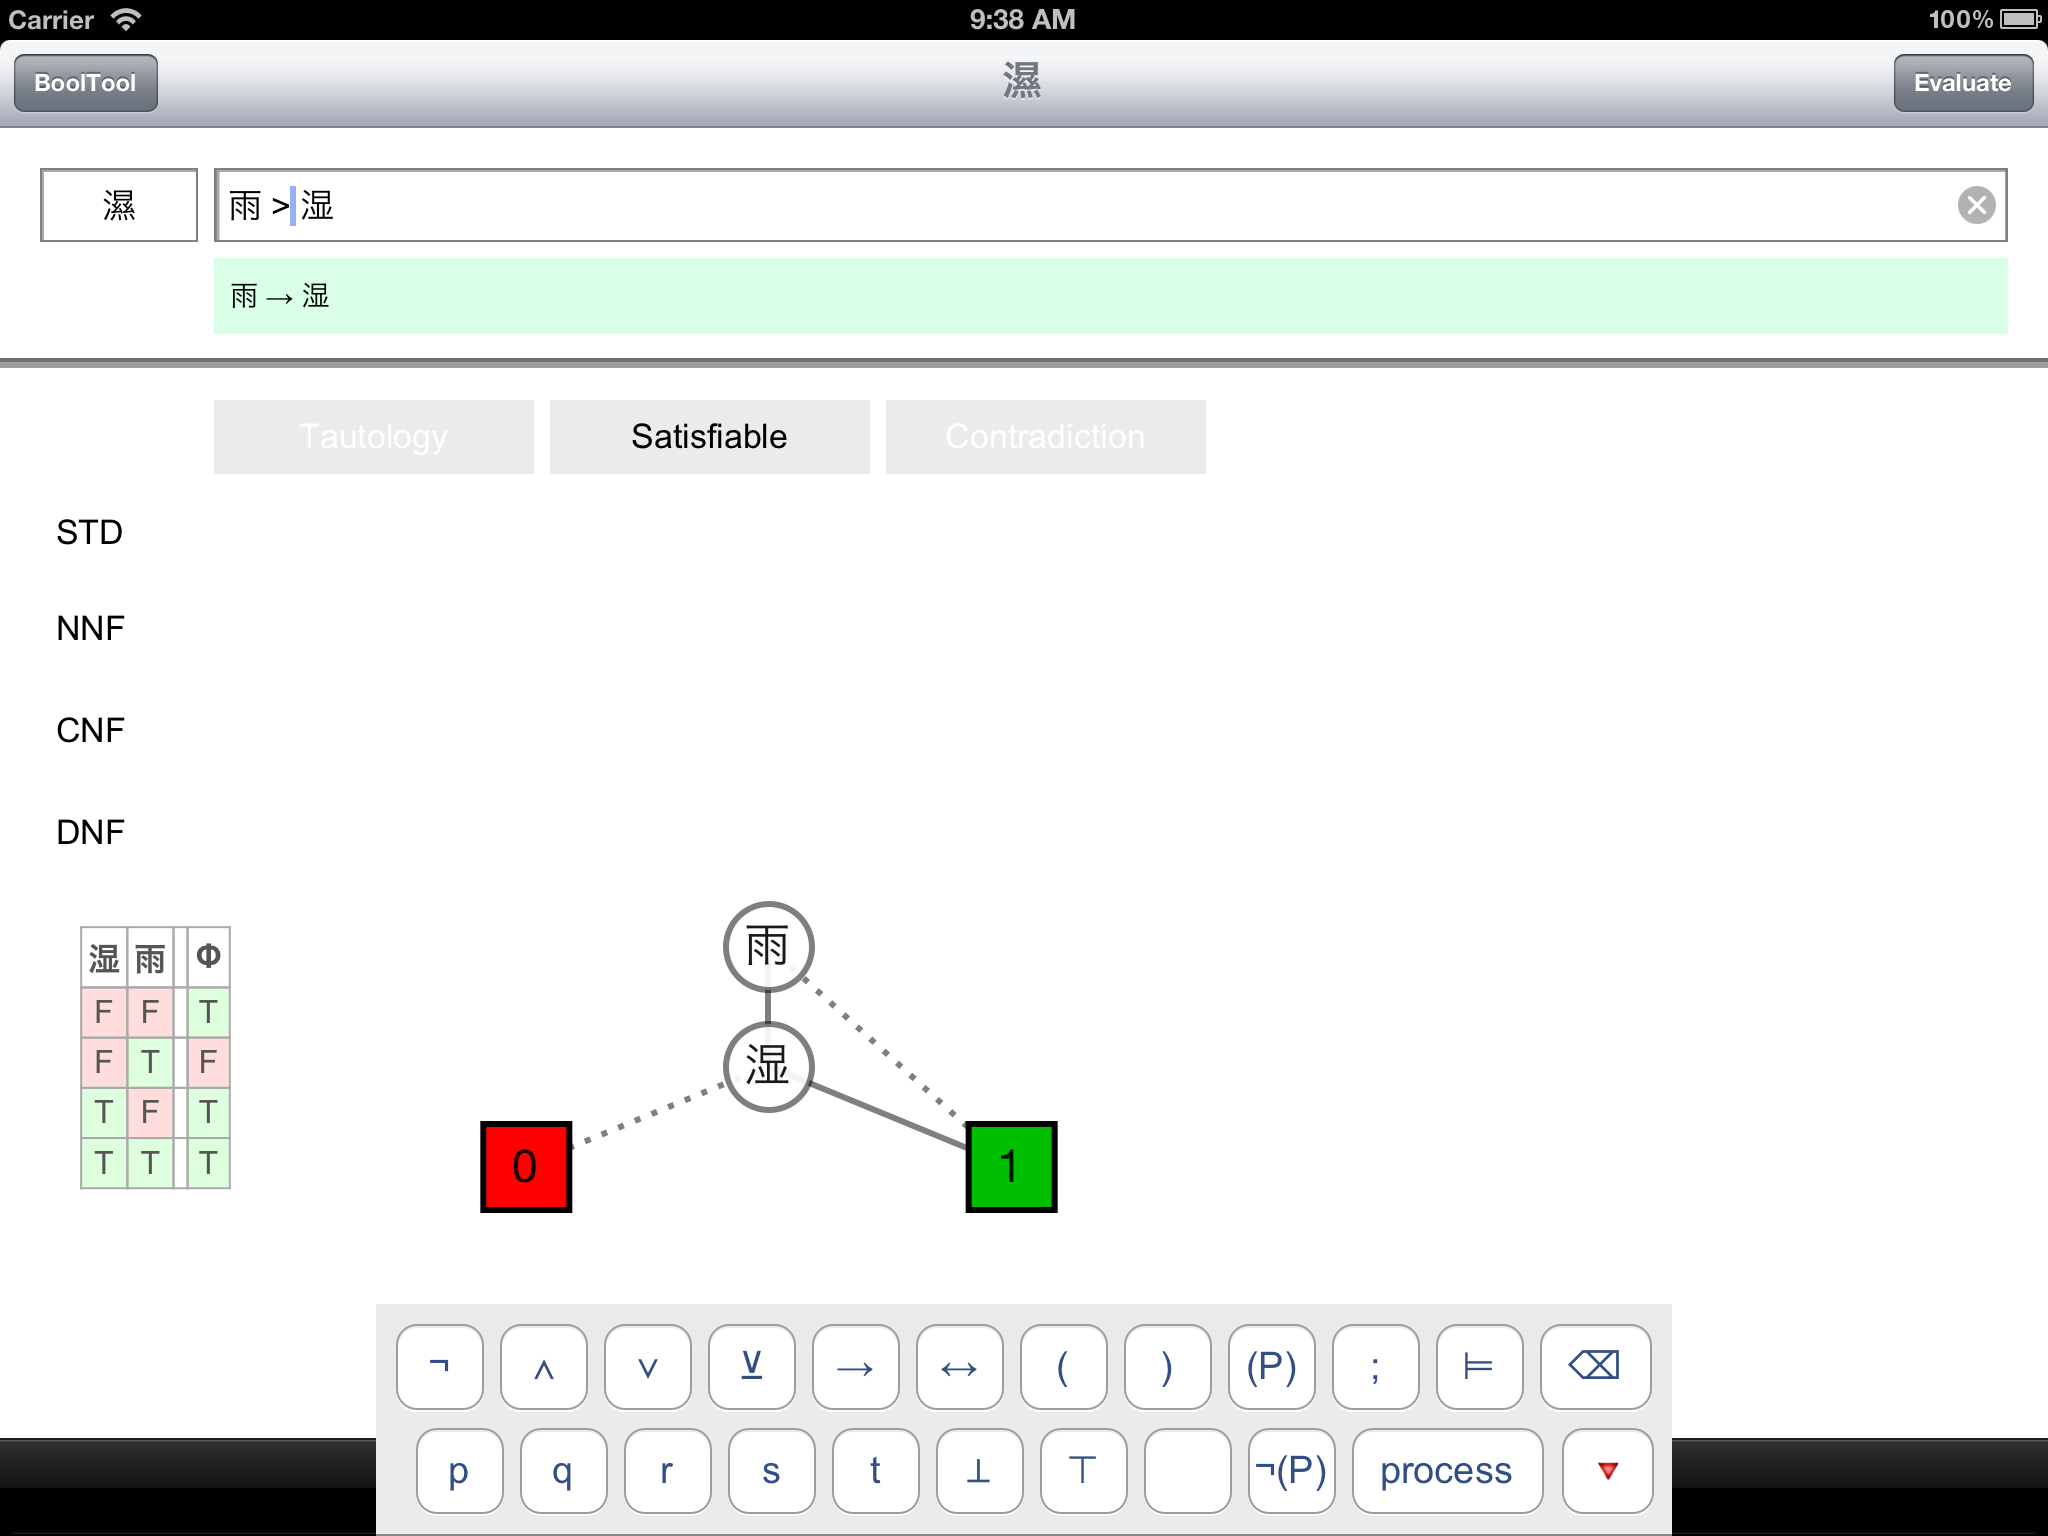
\includegraphics[scale=0.18,trim=0 43cm 0cm 0, clip=true]{concept/RainHD.png}
\caption{Implication with Chinese symbols for rain and wet}
\label{fig:BoolToolChineseInput}
\end{center}
\end{figure}

% ⊨|⊤|⊥|¬|!|∧|&|\\.|∨|\\+|\\||=|↔|<>|→|>|⊻|⊕|\\^|\\(|\\)|,|;|\\w+

\subsection{Output}

BoolTool calculates validity and satisfiability, 
conjunctive normal form, 
disjunctive normal form, 
truth table and 
(reduced) ordered binary decision diagram 
of user's input (\figref{fig:BoolToolROBDD}). 

\begin{figure}[htbp]
\begin{center}
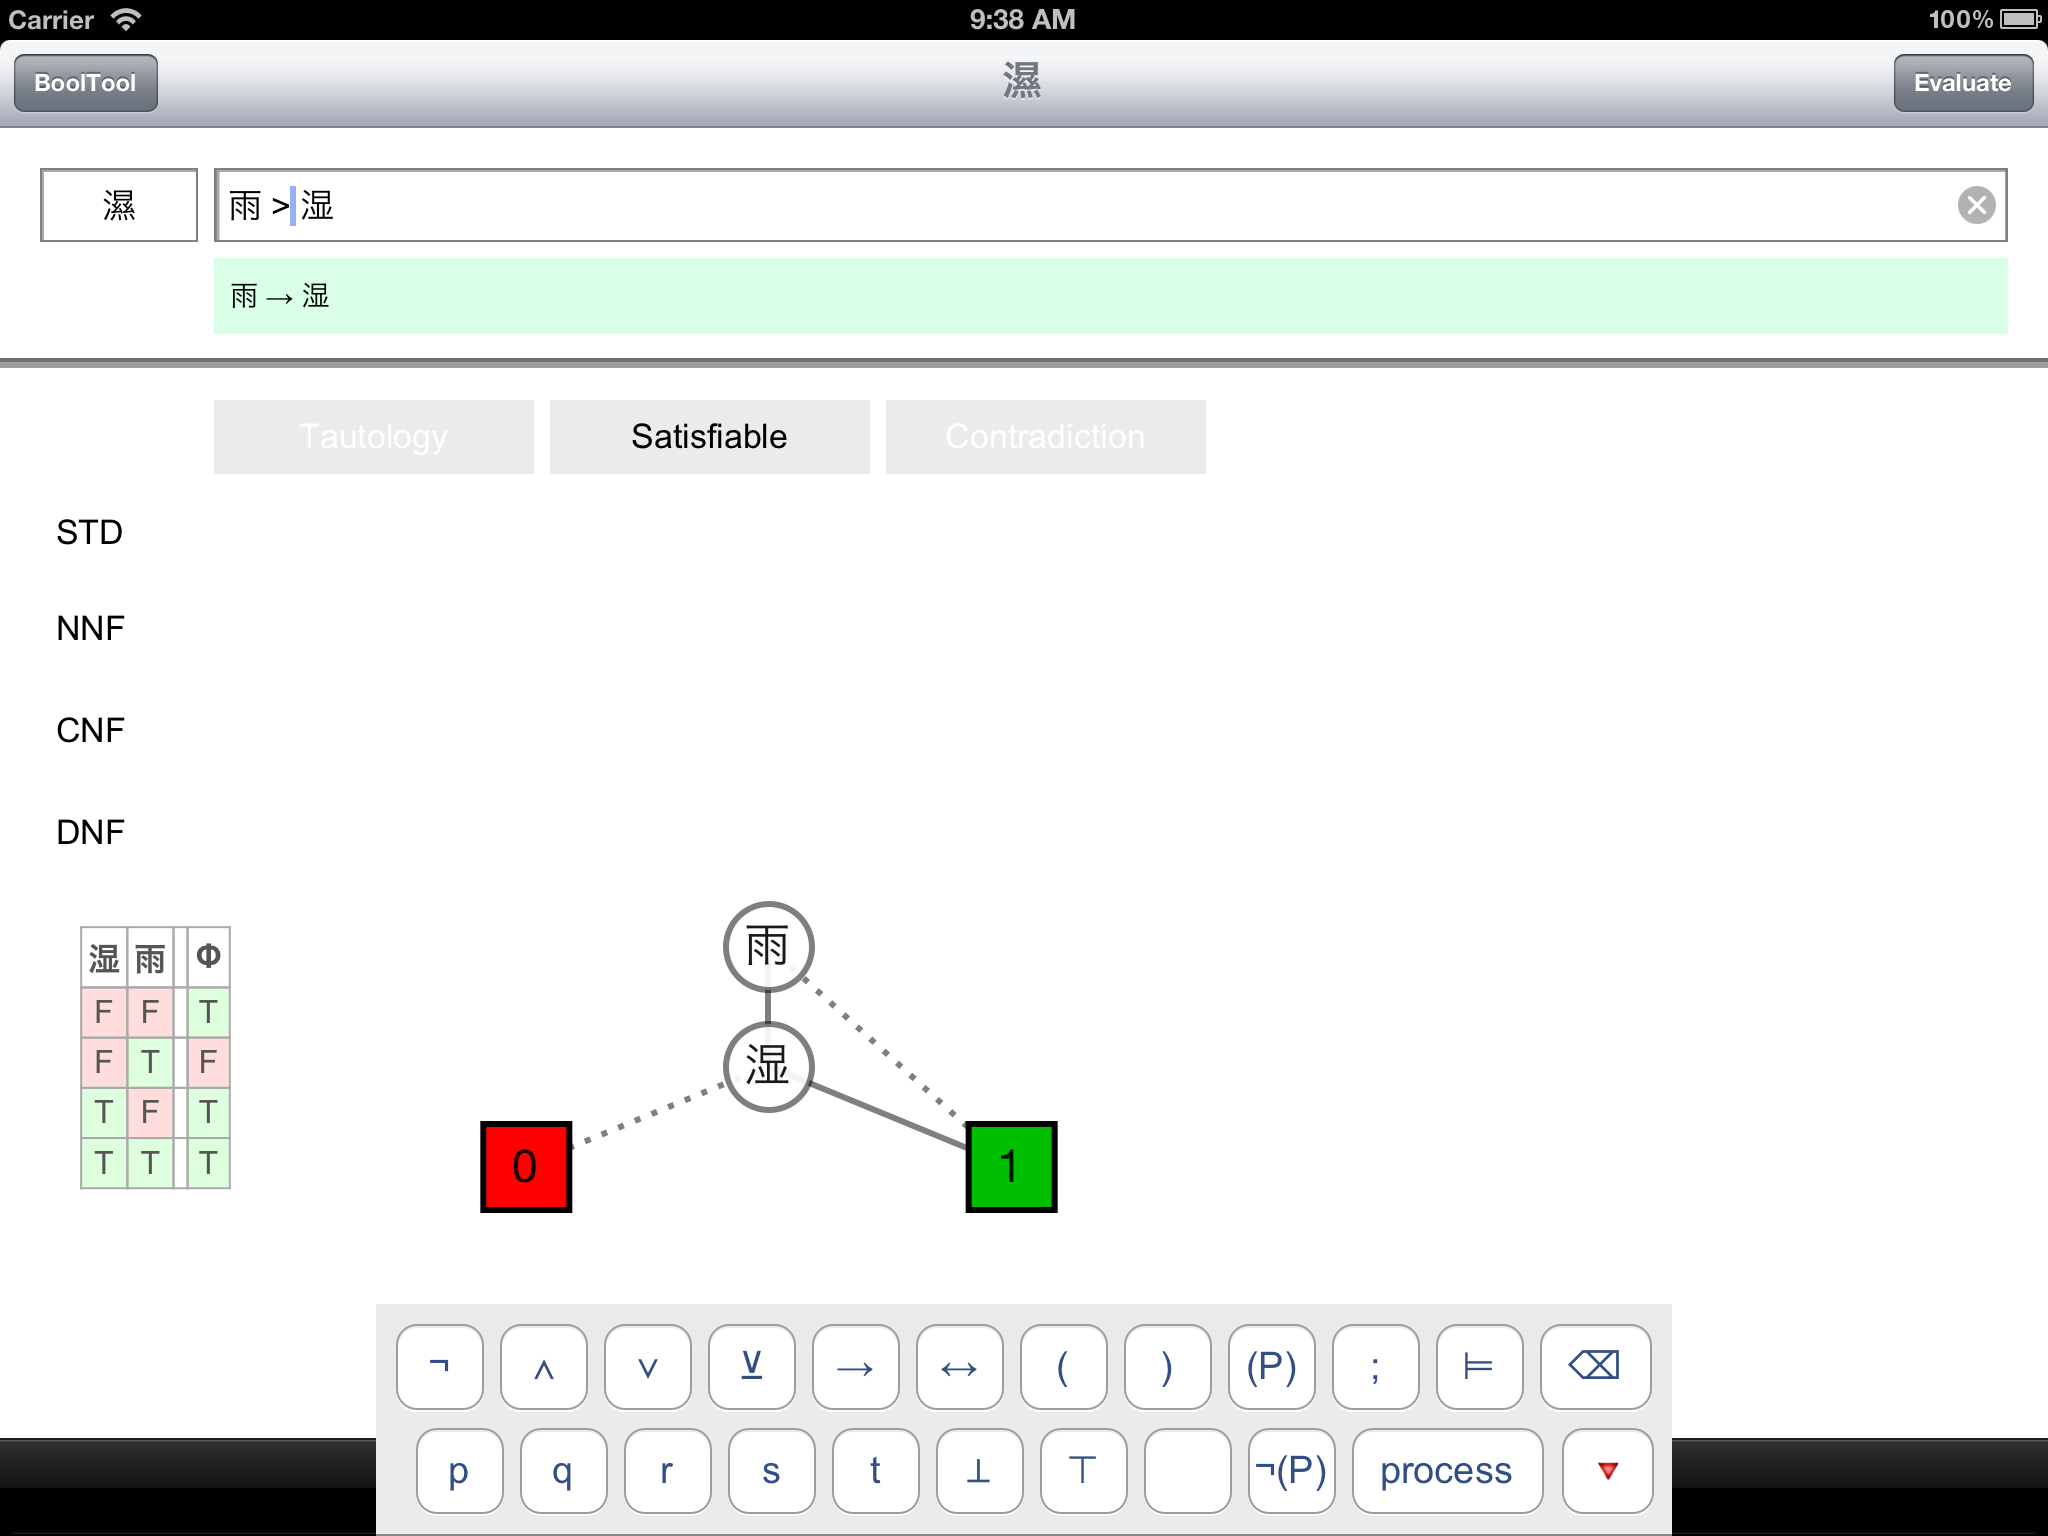
\includegraphics[scale=0.25,trim=16.5cm 11.4cm 34.5cm 31.8cm, clip=true]{concept/RainHD.png}
\caption{Reduced ordered binary decision diagram}
\label{fig:BoolToolROBDD}
\end{center}
\end{figure}

%\begin{figure}[htbp]
%\begin{center}
%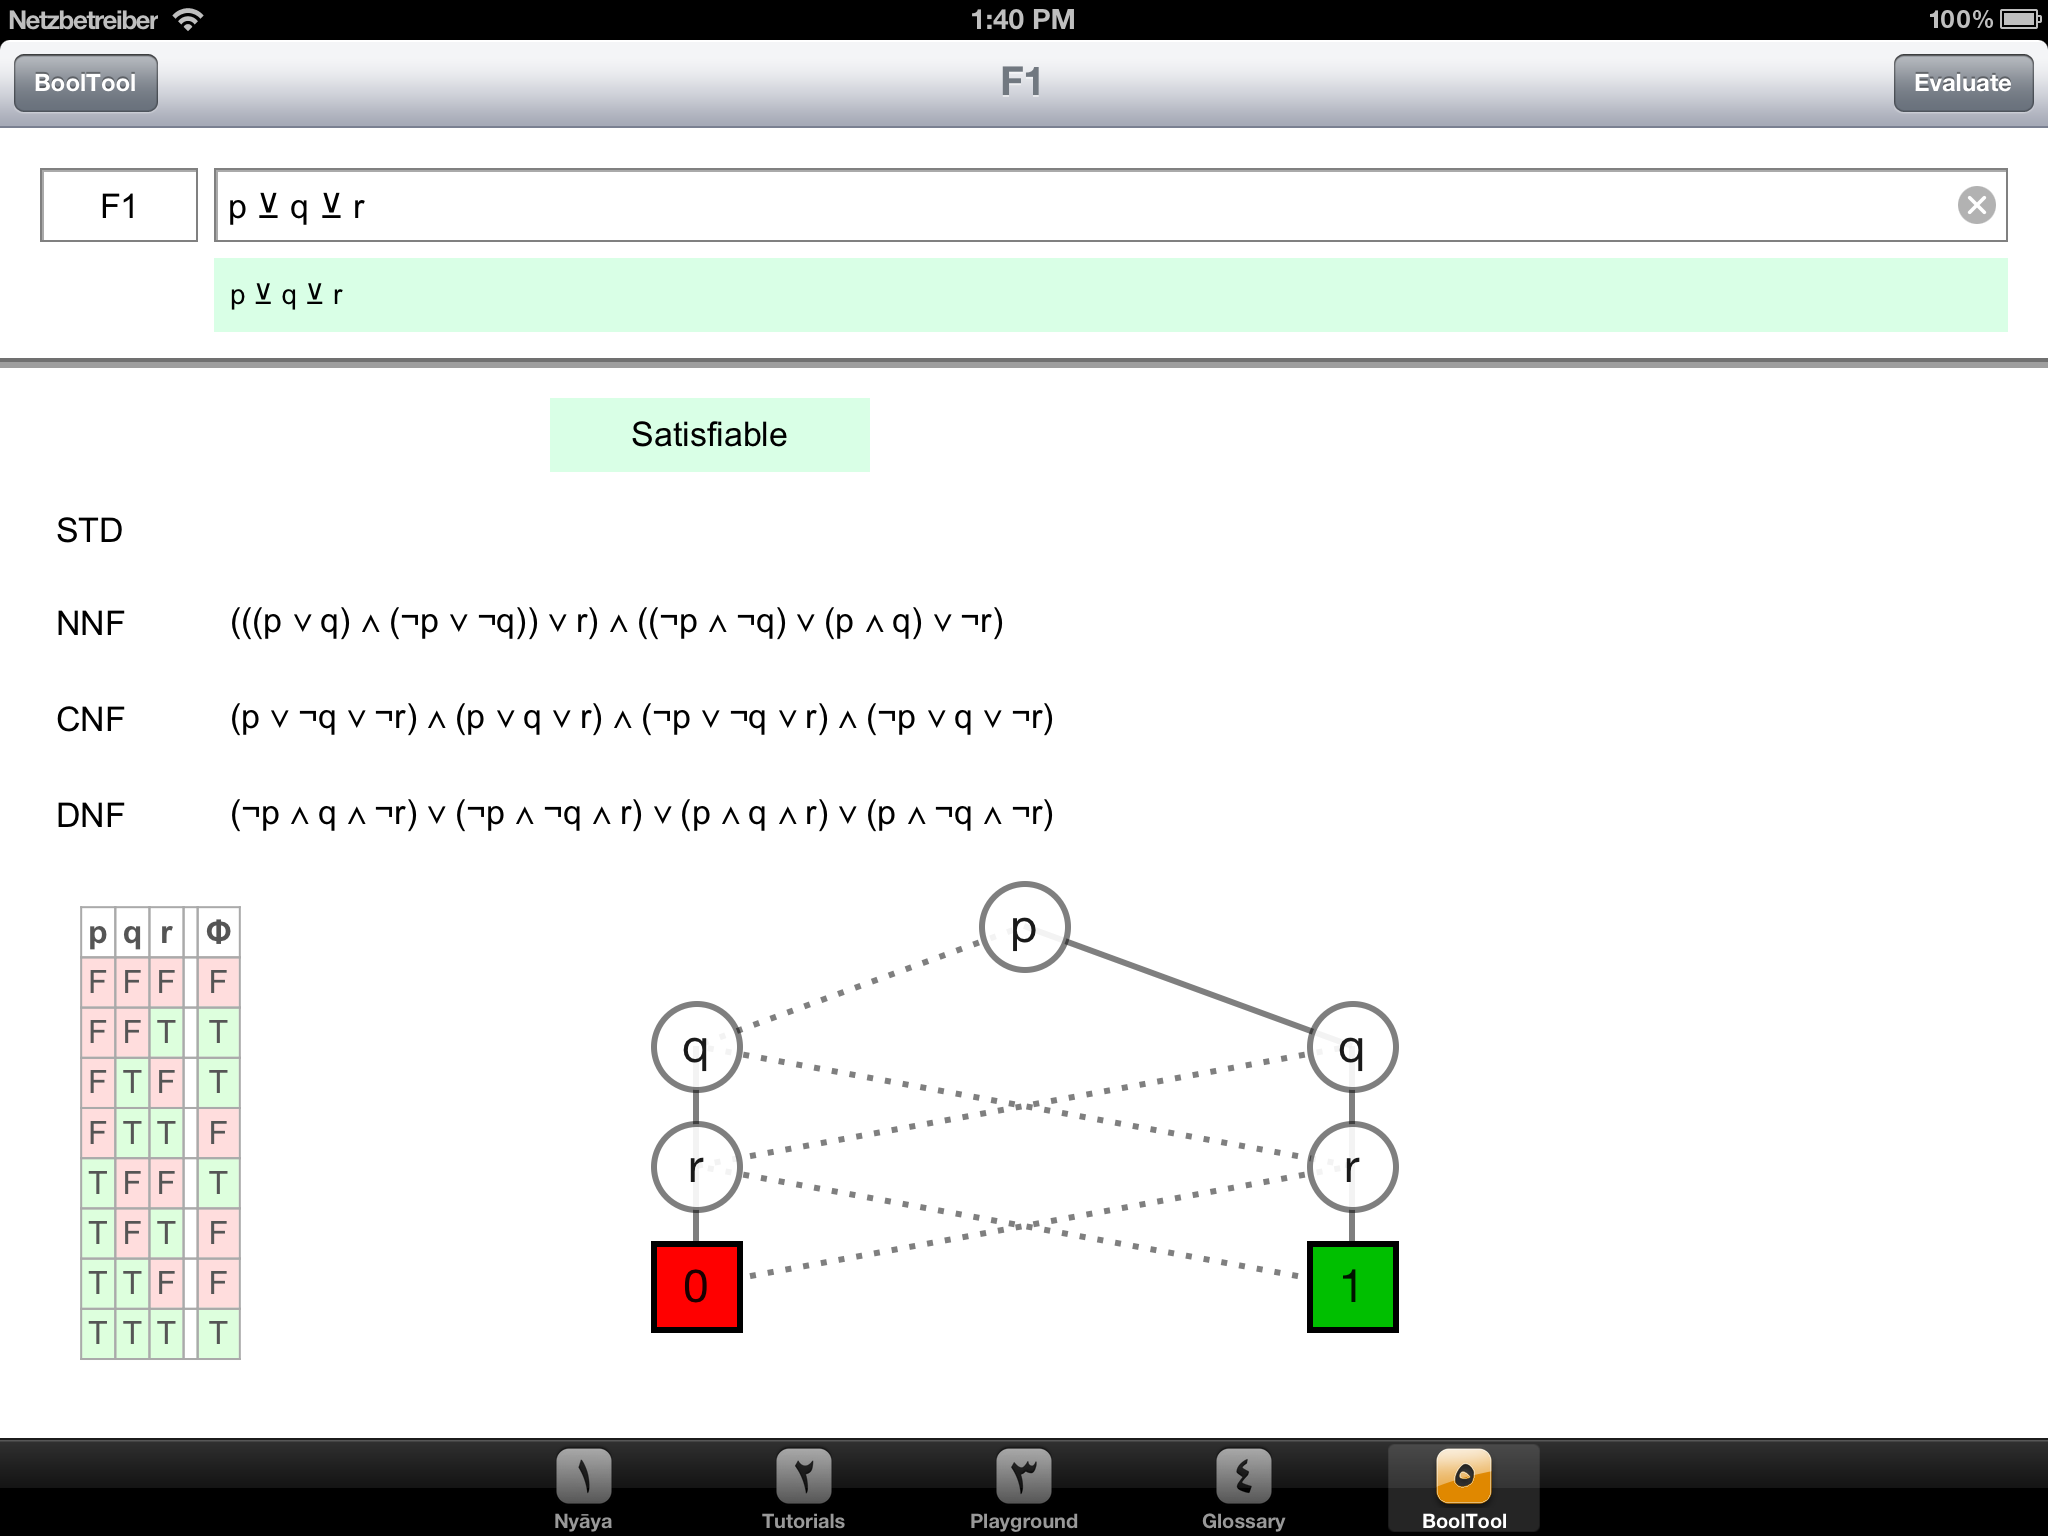
\includegraphics[width=13cm]{concept/BoolTool.png}
%\caption{Boolean function $p \oplus q \oplus r$}
%\label{fig:BoolToolOutput}
%\end{center}
%\end{figure}





\chapter{Tools and Processes}					
% 4 pages
% !TEX encoding = UTF-8 Unicode

\section{Tools}

\subsection{Developing for the iPad}

First steps in developing applications for iPad can be made on a computer running Mac OS X (OS) and 
\href{sec:Xcode}{Xcode} (IDE), which is a free download from the Mac App Store.
Knowledge of object-oriented programming, object-oriented design patterns, 
and the C programming language 
constitutes a good basis to learn the main platform-specific technologies 
\href{sec:ObjC}{Objective-C},
\href{sec:Cocoa}{Cocoa}, and
\href{sec:MemoryManagement}{memory management}
with automatic reference counting.

In addition to the technical skills, an overview of the necessary steps for 
\href{sec:DAD}{Development and Distribution} (p.~\pageref{sec:DAD}) for the iPad platform
should be obtained.

\paragraph{Xcode}
\label{sec:Xcode}
is Apple's integrated development environment to create software for OS X and iOS devices.
It includes an iPad simulator, complete API documentations and development guides to various topics. 
Xcode supports the source management systems Git and Apache Subversion. 
Git will be installed along various other development tools with Xcode.

\paragraph{Objective-C}
\label{sec:ObjC}
is a reflective, object-oriented extension of the C programming language,
which was developed by Tom Love and Brad Cox in the early 1980s (a few moments earlier than C++). 
The syntax for objects and methods is based on Smalltalk. 
Objective-C method calls will be bound to functions at runtime with no need to be defined formally at compile time.
Objective-C code is organized in header \verb=*.h= and implementation \verb+.m+ files 
with \verb+@interface+ and \verb+@implementation+ sections for
the declaration and definition of classes, properties, fields and operations.
The Objective-C keyword \verb+@interface+ must not be mixed up with the Java/C\# \verb+interface+ directive. 
The latter one corresponds to \verb+@protocol+.

\paragraph{Cocoa Touch}
\label{sec:Cocoa}
is the name for the object-oriented APIs for iOS (the operating system for iPhone and iPad). 
Cocoa Touch covers the platform specific Objective-C runtime and a platform specific set of libraries, the frameworks.

\begin{itemize}
\item\label{secitem:CocoaFoundation}
The Foundation framework provides the basis for programming applications in Objective-C. 
In addition to the memory and exception handling it includes the base classes for strings, values, lists, sets and files.
\item\label{secitem:CocoaUIKit} The UIKit framework provides a set of classes and functions for implementing (touch based) graphical user interfaces. 
The architecture of this framework follows the Model-View-Controller pattern 
and the implementation provides a myriad of view and controller classes.
\end{itemize}

\paragraph{Memory Management} 
\label{sec:MemoryManagement}
by the Objective-C run time is based on reference counting. 
The run time does not offer  garbage collection – which is surprising and annoying specifically for Java or C\# developers. 
But the necessary retains and releases are added automatically at compile time.
Most of the time memory management by automatic reference counting is as easy to use as garbage collection.
But one important consequence is that strong object graphs must be implemented as directed acyclic graphs. 
For example, a circular strongly linked list would never be released. 

The advantages are the deterministic and economical run-time behavior.
Objects are destroyed at a defined time and there is no need for a separate thread for garbage collection. 
The main disadvantage is that deallocated objects can still be referenced, 
which would corrupt the event loop
without the possibility of error recovery by exception handling.


%These were very important features in 2007, when the original iPhone was introduced, because
%the hardware for mobile devices was very limited, but looses importance every year.

\paragraph{Development and distribution}
\label{sec:DAD}
for Apple's platforms includes the coding effort and expenses for administration and configuration. 
To install software on iOS devices – especially for distribution via the App Store – applications must be cryptographically signed. 
The necessary certificates are created in the paid members section on Apple's Developer Portal. 
Certificates, development and distribution profiles contain a bunch of identifiers for the identification and differentiation of developers (Team ID), 
applications (App-ID) and a list of permissions (entitlements). 

\subsection{Source Code Management}
\label{sec:SCM}

Every software project includes the need for source code management,
which minimizes the risk of losing working code
by human error or technical failure.
This should be done by powerful, yet lightweight tools.



\paragraph{Git \cite{Git:Main}}
\label{sec:GIT}
is a distributed source code management and revision control system 
- originally developed by Linus Torvalds for Linux kernel development.
Git supports local repositories with full source code history for development.
Local repositories can be synchronized and merged with remote repositories for collaboration and backup
\cite{Chacon:2009:PG:1618548}.

Since Apple's IDE Xcode works with Git's local repositories out of the box,
it was obvious to use Git as source control for the project.

\paragraph{GitHub \cite{GitHub:Main}}
\label{sec.GITHUB}
is a hosting service for projects that use Git. 
GitHub offers free accounts for public repositories, 
which can be seen and downloaded by anyone
using a web-browser or a Git client.
Committing changes is restricted to users chosen by the owner of the repository on GitHub.


As \Nyaya is a student project and the source code should be publicly accessible,
GitHub seemed suitable to house the project.

\section{Project execution}

Projects with only one developer are easy to manage, 
because all work must be done by the same person
and there is no coordination overhead.
Nevertheless small projects need some structure too for a successful outcome.

\subsection{Phases}

The development of \Nyaya for iPad was roughly divided into four phases,
which are substantially coincident with four check-in blocks (see \figref{fig:GitHubGraphAddDel}).

\paragraph{Exploring user interface capabilities.}

After the informal specification of the feature set and the initial presentation of the project
the capabilities of graphical visualization and  user interaction were explored on iPad.
In this phase several prototypes were developed for interactive syntax trees and exercises.

\begin{figure}[htbp]
\begin{center}
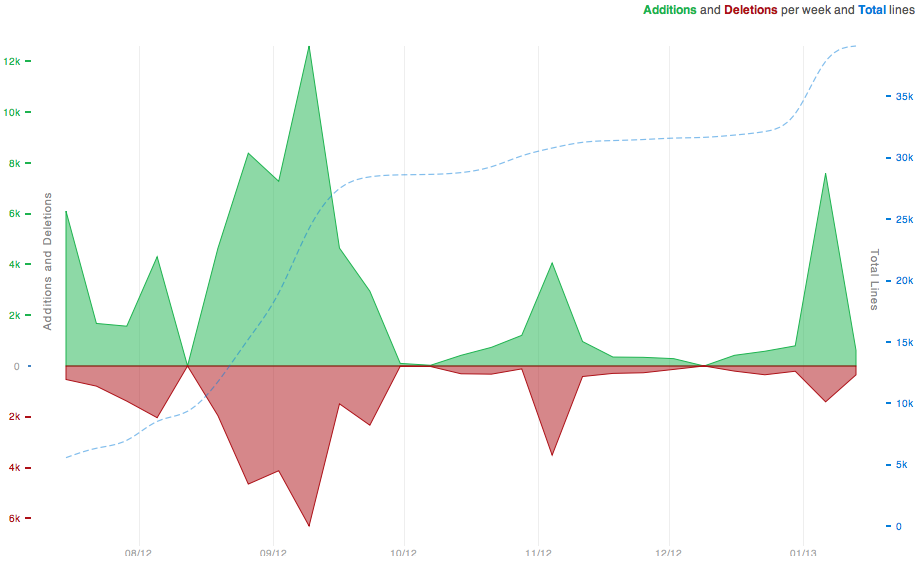
\includegraphics[scale=0.41]{pics/work.png}
\caption{Additions and deletions per week on GitHub}
\label{fig:GitHubGraphAddDel}
\end{center}
\end{figure}

\paragraph{Developing core components.}

%Summer 2012 – Development of the Concept, Include Parser, data structure for AST, BDD

After the formulation of the general concept with tutorials including 
exercises, a playground, a glossary, and the embedding of BoolTool,
the main classes for the representation of abstract syntax trees and binary decision diagrams were implemented.
After several failed attempts to cross-compile \verb=BoolTool='s \verb+OCaml+ sources 
and to use the binaries on iPad, the functionality of \verb+BoolTool+ was reimplemented as \BoolTool in Objective-C.
% A left recursive descendent parser for input strings with the syntax propositional logic was implement in Objective-C. 
The additional workload was rewarded by a more flexible parser than CL \verb+BoolTool+’s parser.
The parser accepts standard symbols of propositional logic as well as operator symbols of Boolean expressions.
Furthermore, characters and words of all languages can be used as identifiers for atoms.

\paragraph{Adding content, controllers, and configurations.}

Although the general concept was developed, content had to be expanded. 
The tutorials had to be written and the exercises had to be generated. 
Content and configuration files had to be added to the project. 
The different views had to be controlled and the navigation between the different use cases had to be added. 

\paragraph{Finishing.} In the final phase all parts of the program were reviewed.
\Nyaya's content was amended and this document was written. 
\Nyaya was prepared for distribution in the App Store.

\subsection{Development model}

The development of this software did not follow a specific development model, 
but did borrow some principles from agile development.

\paragraph{Fail-Fast.} The interaction with syntax trees and 
the integration of \verb=BoolTool= were identified as essential parts with a high risk potential. 
The first one was cleared by exploring the user interface capabilities.
The second one failed at the beginning of developing core components 
and was substituted with a native implementation of the functionality of \verb=BoolTool=
under direct control of the project.

\paragraph{Test-driven development.}

Parsers, trees and operations on trees were the ideal application for test driven development.
First, the expected results were defined in test cases, then the functionality was implemented.
So it was ensured that at every point of the development cycle 
the core of the application was still working as defined,
when all unit tests had succeeded.

\paragraph{Refactoring.}
Due to occurring memory and performance issues on the iPad
some implementations had to be reconsidered 
and some functionality had to be reimplemented.
This could be done without complications because 
the local repository provided a complete development history 
and unit tests provided a quick check, whether the reimplementation was correct.

\paragraph{Use cases.}
With the written concept (see chapter \vref{ch:concept}) of an interactive environment for BoolTool 
that enables the learning  of simple facts about propositional logic the collection of use cases was defined. 
These use cases represent the real value of the project 
and they define the criterion for completion of development.



\chapter{Implementation}						
% 10 pages
% !TEX encoding = UTF-8 Unicode
% ÄÖÜ ß äöü

\section{Architecture}

The general design of \Nyaya follows the Model-View-Controller pattern,
which is originated in Smalltalk \cite[p.4]{GAMMAETAL}, 
that separates the representation of data from the user interaction.
Cocoa Touch \seeref{sec:Cocoa} encourages the use of MVC 
by providing a rich set of useful views and controllers with the framework UIKit.
Those cover many use cases of data presentation and user interaction.

\section{Model}

\Nyaya must hold different representations of Boolean functions – propositional formulas, abstract syntax trees and binary decision diagrams. 

\subsection{Propositional formulas and Boolean expressions}
Since propositional formulas and Boolean expressions are subsets of the set of all Unicode strings,
they are easily represented by the standard string classes of actual frameworks. 

Due to the unambiguous relationship between propositional formulas and Boolean expressions 
\Nyaya allows the use of a mixed syntax and additional symbols as input
for the user's convenience. The input expression $!a \wedge b + c \oplus a$ translates into the propositional formula
$\neg a \wedge b \vee c \veebar a$ (see \vref{subsec:Parser}).

\subsection{Abstract Syntax Trees}

Cocoa does not provide a class to represent trees, 
but with instances of a class, 
that implements the composite pattern \cite[p.163ff]{GAMMAETAL}
arbitrary graphs and therefore syntax trees can be represented easily.

\begin{figure}[htbp]
\begin{center}
\UML{NyayaNode.png}
\caption{Node class to represent an abstract syntax tree}
\label{fig:NyayaNodeCluster}
\end{center}
\end{figure}

\subsubsection{Node class cluster}

The node class is implemented as a class cluster, 
which is an Cocoa design pattern \cite[p.282ff]{Buck:2009:CDP:1803585}
– an adaption of the the abstract factory design pattern \cite[p.87ff]{GAMMAETAL}.
The abstract and public class \verb+NyayaNode+ 
provides a set of static and public methods (see \figref{fig:NyayaNodeCreation}),
that returns instances of non public sub-classes (see \figref{fig:NyayaNodeCluster})
of \verb+NyayaNode+.

\begin{figure}[htbp]
\begin{center}
\UML{NyayaNodeCluster.png}
\caption{Public root class and non public subclasses}
\label{fig:NyayaNodeCluster}
\end{center}
\end{figure}

Actual the creational methods were implemented as a class category in a different source file. 
Class categories are a language feature of Objective-C \cite[p.225ff]{Kochan:2009:PO:1538451}
– an adaption of the decorator design pattern \cite[p.175ff]{GAMMAETAL} – 
to extend or organize the functionality of given classes beyond their core purpose. 

There are base implementations of category methods in the root node class,
that will be overridden in subclasses.
For example \verb+isLiteral:bool+ returns false for all node instances
except for instances of variables
and instances of negations of variables.

The variable node class adds setters for the categories \verb+Valuation+  (\figref{fig:NyayaNodeValuation})
and \verb+Display+.

\subsubsection{Node class categories}

\begin{itemize}

\item The category “Creation” implements the production rules of the grammar 
to create syntax trees recursively (\figref{fig:NyayaNodeCreation}).
Since the constructors of all classes in the cluster are hidden, 
the production of invalid syntax trees is prevented.

\begin{figure}[htbp]
\begin{center}
\UML{NyayaNodeCreation.png}
\caption{Production rules}
\label{fig:NyayaNodeCreation}
\end{center}
\end{figure}

\item The category “Description” provides methods to convert a syntax tree into one of it's string representations – 
either a propositional formula in strict syntax with many parentheses 
or a formula using precedences and associativity.
In most cases, the second form leads to shorter strings with less parentheses. 
In rare case, only the outer parentheses are omitted.

\item The category “Display”  allows extended valuations (undefined, false, true) 
with incomplete truth assignments. 
It is used for the interactive syntax tree view on the playground, 
where the user can assign truth values to some or all atoms.
% (see \figref{fig:NyayaNodeDisplay)


\item The category “Attributes”  provides information about the number of sub-nodes of a node 
and the normal forms the sub-tree matches.

\item The category “Transformations” provides equivalence transformations 
and methods to create 
 semantically different syntax trees by replacing atoms, connectives or sub-trees with
atoms, connectives or trees.

\item The category “Derivations” defines methods to derive semantically equivalent normal forms from a given syntax tree.

\item The category “Random” creates arbitrary syntax trees with a given set of connectives and atoms and within a range for the number of nodes. It is used to create formulas for the exercises.

%\item The category “Reductions”
%\item The category “Resolution”
\item The  category “Type” provides one method, that returns the type of a node, i.e constant, variable, type of connective as an enum.


\item The category “Valuation” (\figref{fig:NyayaNodeValuation}) 
provides fast valuations with complete truth assignments. 
It is used to create truth tables and binary decision diagrams. 

\begin{figure}[htbp]
\begin{center}
\UML{NyayaNodeValuation.png}
\caption{Valuation of trees}
\label{fig:NyayaNodeValuation}
\end{center}
\end{figure}

\end{itemize}
\subsubsection{Immutable syntax trees}

Instances of node classes are not mutable 
regarding their function as nodes of abstract syntax trees. 
This means nodes can be created, but not modified.
The symbol of an atom can not be changed, 
a connective node can not be altered into an other one,
and child nodes of a connective node can not be replaced or reordered.

Derivations or transformations do not change the structure of an existing syntax tree,
but rather create a new independent syntax tree.

Obviously mutable truth assignments does not affect the immutable structure of a syntax tree,
because truth assignments are semantics, not syntax. 

\subsubsection{Acyclic syntax graphs}

Since the representation of abstract syntax trees is implemented immutable,
there is no need to create multiple instances for syntactically equivalent sub-trees. 
At run-time syntax trees are represented by acyclic syntax graphs, 
where multiple sub-trees can be represented by the same instance-graph
(\figref{fig:AST+ASG}).

\begin{figure}[htb]
\begin{center}
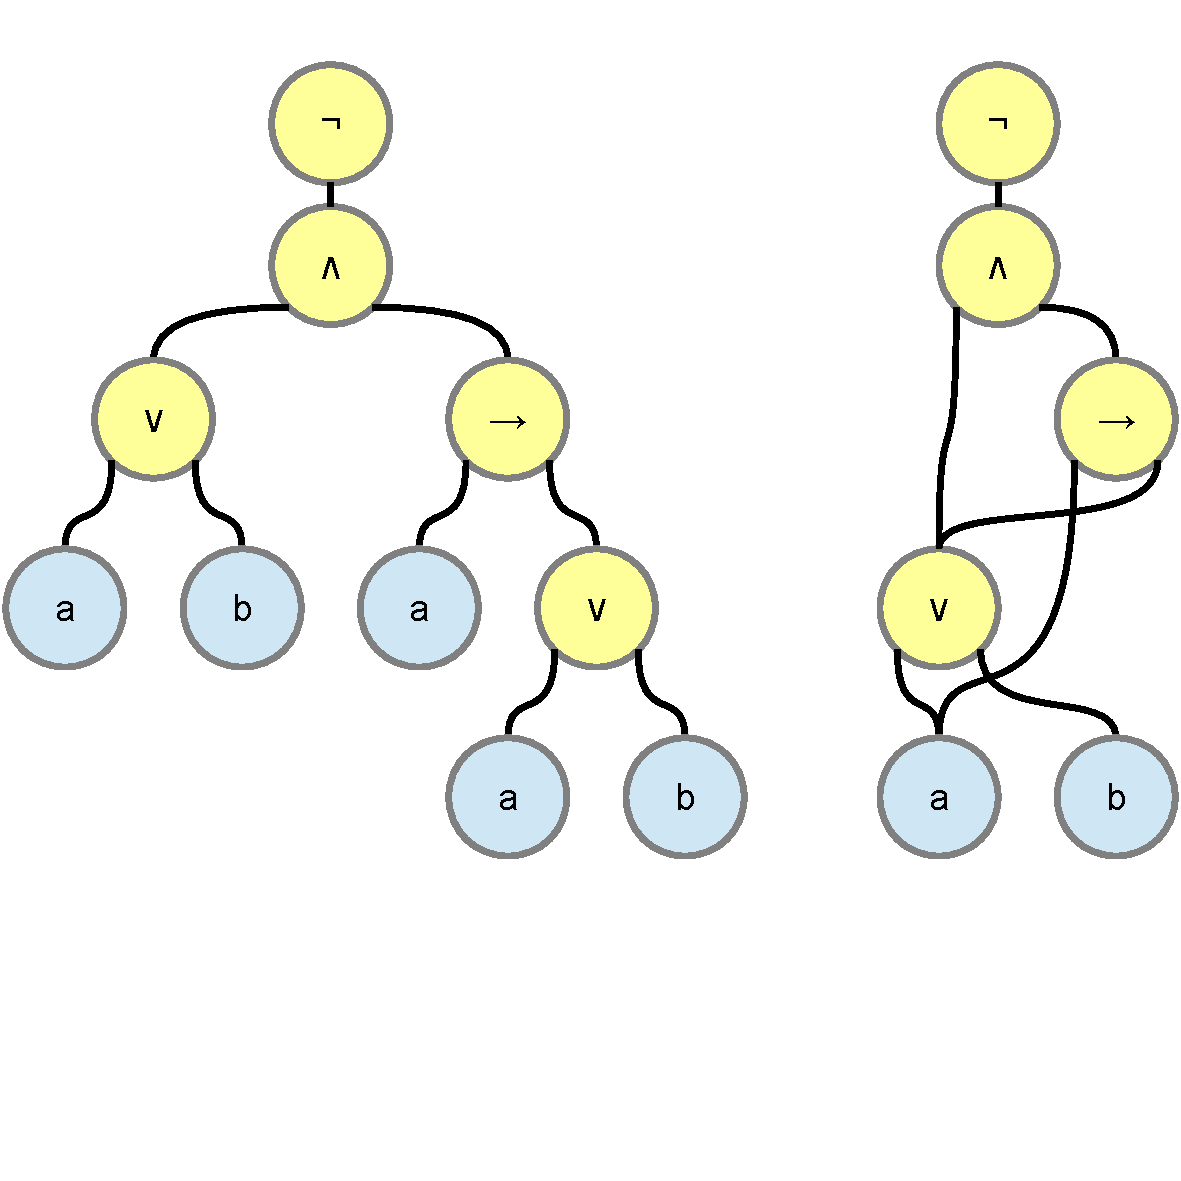
\includegraphics[scale=0.5,trim=0cm 5.4cm 0cm 1cm,clip=true]{diagrams/AcyclicSyntaxGraph.pdf}
\caption{Abstract syntax tree – acyclic graph }{$\neg( (a\vee b) \wedge (a \rightarrow a\vee b))$}
\label{fig:AST+ASG}
\end{center}
\end{figure}

This eases the detection of obvious tautologies $P \vee \neg P$, $P \rightarrow P$ and contradictions $P \wedge \neg P$,
because the sub-tree $P$ on the left side is represented by the same object-graph as the sub-tree $P$ on the right side.

\subsubsection{Limitations}

The derivation of normal forms will fail on some relatively small syntax trees.
especially when the formula contains too many exclusive disjunctions.

With every exclusive disjunction of a formula $P$ and an atom $p$, 
that is not already used in $P$,
the number of nodes will at least double 
when deriving an equivalent implication free form.
“Implication free” means also the absence of exclusive disjunctions (see \tabref{tab:BNFGRIFF}).

\begin{eqnarray*}
\#(P \oplus p) & = & 1 \cdot(\#(P) + 2) \\
\#((P \wedge \neg p) \vee  (\neg P \wedge p)) & = & 2 \cdot (\#(P) + 2) + 3 \\
\#((P \vee p) \wedge  (\neg P \vee \neg p)) & = & 2 \cdot (\#(P) + 2) + 3 \\
\end{eqnarray*}

The syntax tree for an exclusive disjunction of 20 different atoms is build from 39 nodes.
The syntax tree of a semantically equivalent implication free form will already contain over four million nodes.
Deriving the negation normal form does not increase or decrease the number of nodes significantly,
but the necessary distributions of disjunctions will multiply the number of nodes again.

To ensure the stability of \Nyaya 
and since it is near impossible 
to present a propositional formulas with thousands of symbols 
to the user in a meaningful way, 
the derivation of normal forms is aborted, when the results surpass a defined size.



\subsection{Parser}
\label{subsec:Parser}

The backend of \verb+BoolTool+\footnote{
\href{http://cl-informatik.uibk.ac.at/software/booltool/}{cl-informatik.uibk.ac.at/software/booltool/}} 
– parsing and transformation of Boolean functions – 
is implemented in \verb+OCaml+\footnote{
\href{http://ocaml.org}{ocaml.org}}, 
a functional programming language, which is well suited for this kind of task.

After several failed attempts to cross-compile the \verb+OCaml+ sources to iPad's processor architecture (ARM),
to link the object code to the Xcode project and to bridge and call functions from C, 
the implementation of a simple translator 
for propositional formulas (a subset of all possible strings)
into syntax trees looked more promising. 

The generation of a syntax tree from a formula  is carried out in two steps. 

\subsubsection{Scanning}

In the first step the input string is transformed into an array of strings – the list of input tokens –
using the standard regular expression class of Cocoa Foundation.
\begin{table}[htdp]
\begin{center}
$\top | \bot 
| \neg | !
| \wedge | \& | .
| \vee | {\setminus}| | {\setminus}+ 
| \veebar | \oplus | \textasciicircum
| = | <> | \leftrightarrow 
| > | \rightarrow | \models
| ( | ) | , | ; 
| {\setminus}w+$ 
\caption{Regular expression for the scanner}
\label{tab:REGEX}
\end{center}
\end{table}

The set of valid tokens, which includes identifiers, connectives and parentheses
was simply defined by writing a suitable regular expression (see \tabref{tab:REGEX}), 

\subsubsection{Parsing}

In the second step the list of input tokens is parsed top-down 
using a recursive-descent parsing algorithm \cite[p.144ff]{Louden:1997:CCP:523017} 
following an ebnf grammar outlined in \tabref{tab:CoreEBNF}), 
that defines precedence and associativity of connectives too.

\begin{table}[htdp]
\begin{center}
\begin{lstlisting}[mathescape]
formula        ::= entailment
entailment     ::= sequence [ '$\models$' entailment]
sequence       ::= bicondition { ';' bicondition } 
bicondition    ::= implication [ '$\leftrightarrow$' bicondition ]
implication    ::= xdisjunction [ '$ \rightarrow$' implication ]
xdisjunction   ::= disjunction { '$\veebar$' disjunction }
disjunction    ::= conjunction { '$\vee$' conjunction }
conjunction    ::= negation { '$\wedge$' negation }
negation       ::= '$\neg$' negation | '(' formula ')' | identifier
\end{lstlisting}
\caption{Core EBNF grammar for the parser}
\label{tab:CoreEBNF}
\end{center}
\end{table}

\subsubsection{Limitations}

\Nyaya does not parse as fast and (memory) efficient as BoolTool's parser,
primarily because recursion and token probing are more expansive operations in Objective-C than in OCaml.
The creation of a syntax graph instead of an syntax tree adds more overhead.
But \Nyaya's implementation is {\em good enough}, 
because {\em real world} user input is limited to at most few thousands characters.

Unit tests has shown that the there are no memory or run-time issues, 
although the parsing can take a second or two on an iPad.

\subsubsection{Enhancements}

Despite the drawbacks mentioned above
the benefits far outweigh the disadvantages of implementing an own parser.

\begin{itemize}

\item \Nyaya parses strings with Unicode characters, 
therefore identifiers are not limited to Latin letters and
$\alpha + \omega$ will be parsed correctly. 

\item The grammar rules for operators are defined as sets of tokens, 
which will be initialized at application start. 

\begin{table}[htdp]
\begin{center}
\begin{lstlisting}[mathescape,firstnumber=7]
disjunction    ::= conjunction { OR conjunction }
\end{lstlisting}
\begin{lstlisting}[mathescape,firstnumber=15]
OR             ::= '$\vee$' | '$|$' | '$+$' | 'O'
\end{lstlisting}
\caption{Excerpts from a localized grammar (Italian)}
\label{tab:LocalizedEBNF}
\end{center}
\end{table}
% conjunction    ::= negation { AND negation }
% AND            ::= '$\wedge$' | '$.$' | '$\&$' | 'E'

\item Symbols for operators
can be localized using the standard localization framework of Cocoa.

\begin{table}[htdp]
\begin{center}
\begin{lstlisting}[mathescape,numbers=none,multicols=2]
IMP = "$\rightarrow$ $>$ IMPLIES";
OR  = "$\vee$ | + OR";
AND = "$\wedge$ & . AND";
NEG = "$\neg$ ! ~ NOT";
IMP = "$\rightarrow$ $>$ IMPLICA";
OR  = "$\vee$ | + O";
AND = "$\wedge$ & . E";
NEG = "$\neg$ ! ~ NON";
\end{lstlisting}
\caption{Localizable.strings in en.lproj and it.lproj}
\label{tab:LocalizableStrings}
\end{center}
\end{table}


\item The parser generates syntax graphs with objective-c run-time objects,
which are well suited for the use cases in an interactive environment.

\end{itemize}

\subsection{Truth Tables}

Truth tables are either small enough to be computed on demand or too big to be stored in memory.
Either way there is not reason to store filled truth tables at run-time.

\subsection{Binary Decision Diagrams}

Binary decision trees and diagrams are represented by trees 
or acyclic directed graphs built from instances of a simple node class
 with attributes for a name, a left branch and a right branch. 
\begin{table}[htdp]
\begin{center}
\UML{BddNode.png}
\caption{Attributes and factory method of BddNode}
\label{fig:BddNode}
\end{center}
\end{table}
The name is either an identifier, i.e. the name of a variable, “0” or “1". 
Nodes with the name “0” or “1” are leaf nodes or result nodes
and must not have a left or right branch.
The other nodes with the name of a variable are decision nodes 
and must have valid left and right branches. 

The class provides a factory method to create 
(un)reduced ordered binary decision diagrams from abstract syntax trees
(\figref{fig:BddNode}).

\newpage\section{Views and Controllers}

\Nyaya's main navigation – switching between Welcome, Tutorials, Playground, Glossary and NyBoolTool – 
is organized by a sub-class of\verb+ UITabBarController+ (an heir of \verb+UIViewController+). 
At start the tab bar controller will be instantiated and invoked by \Nyaya's application delegate. 
The tab bar controller will present it's \verb+UITabBar+ (an heir of \verb+UIView+)
and will appoint of one of it's view controllers, which will present it's view such as the welcome screen.

Tabbing an \verb+UITabBarItem+ will cause the tab bar to delegate the event to it's \verb+UITabBarDelegate+ – the tab bar controller.
The tab bar controller will switch the selected view controller, which then will present it's content.

Except for the welcome view controller 
all content view controllers inherits from split view controller,
which provides a master view controller and a detail view controller.
The tutorial master view controller and the BoolTool master view controller shares a list of persisted formulas.

\subsection{Welcome}

The welcome view controller is simple subclass of\verb+ UIViewController+ and presents it's content in an not so simple \verb+UIWebView+,
which is a fully functional, but ‘naked’ web-browser, i.e. links are followed and there is a page history, but no back-button is presented.
The behavior of the web view can be altered by implementing a web view delegate – usually the controller.

\subsection{Tutorials}

The tutorials master view controller presents a table view with five sections of tutorials.
The sections organize the tutorial titles for 
introduction, syntax, semantics, normal forms and binary decision diagrams.
Tabbing an entry will cause the detail view controller to present the corresponding tutorial in a web view
with an additional exercise button on the top of the view.

Tabbing this exercise button will put the exercise view controller in charge. 
An suitable overlay view will be opened, 
and an instance of a matched class implementing of\verb+ NyTuTester+ will be created.

\begin{figure}[htbp]
\begin{center}
\UML{NyTuTester.png}
\caption{Tester interface}
\label{fig:Tester}
\end{center}
\end{figure}

The method \verb+firstTest+ initializes the test parameters and fills the test view with instructions and labels. 
Then it calls \verb+nextTest+, which will fill the test view with a new question by every call.
The method \verb+checkTest+ evaluates the user's answer and displays the result in the test view.
When the test view is closed by the user \verb+removeTest+ will dispose resources attached to the test view.

\subsection{Playground}

The playground master view controller presents a table view with the list of stored and selectable formulas.
The user can use a formula from this list to add a tree view to the detail view – the canvas view.
Or the user can add a new tree view by an tap and hold gesture to the canvas view.
The canvas view can hold multiple syntax trees.

\begin{figure}[htbp]
\begin{center}
\UML{TreeView.png}
\caption{Canvas view with multiple syntax tree views}
\label{fig:TreeView}
\end{center}
\end{figure}

The nodes of the syntax tree view are drawn as circles around \verb+symbol()+ 
method defined in the category
\verb+Display+ of the class \verb+NyayaNode+..
The color of the border is determined by the value of \verb+displayValue()+.


\begin{figure}[htbp]
\begin{center}
\UML{NyayaNodeDisplay.png}
\caption{Node display interface}
\label{fig:NyayaNodeDisplay}
\end{center}
\end{figure}

\subsection{Glossary}

The glossary master view controller reads all elements with an id from the glossary content document,
creates an alphabetical ordered list of technical terms using the texts included between the corresponding element-tags.
This list of technical terms defined by the glossary document is presented in a table view.
Tapping a term will scroll the glossary document view – a web view - to the chosen term, 
controlled by the glossary detail view controller.

\subsection{BoolTool}

The BoolTool master view controller presents a table view with stored and selectable formulas.
An editable text field with an attached customized keyboard will allow the user to enter their formulas.

The output will be presented in different views. Read only text views are used for the normal form, 
a web form is used for the truth table and a customized view will draw the binary decision diagram.



%\section{Unit-Tests}
%\newpage
\section{Application content}

Beside the classes to determines the run-time behavior of the application,
the storage of application content must be defined.

\subsection{Content on delivery}

Configuration data, localization data and html documents
are stored in UTF-8 encoded text files.
All graphical content such as icons and diagrams are stored in portable network graphics.
These content files are embedded in \Nyaya's app bundle
and will be downloaded along the application execution data,
while receiving \Nyaya for iPad from the App Store.

\subsection{User created content}

Formulas from the playground and BoolTool are persisted 
in the simple property list file \verb+BoolToolData+ 
in the documents folder of the app.

\subsection{Export and import of content}

Single formulas can be exported from or imported into editable text fields 
by simple using the standard copy and paste mechanism of iOS.






\chapter{Retrospective} 			
% 2 pages
% !TEX encoding = UTF-8 Unicode
% ÄÖÜ ß äöü

\section{Retrospective}

\section{Outlook}






\chapter{Conclusion and Summary}				
% 1 pages
% !TEX encoding = UTF-8 Unicode
% ÄÖÜ ß äöü








%===================================================================
% END: CONTENT -----------------------------------------------------
%===================================================================

\cleardoublepage
\phantomsection
\addcontentsline{toc}{chapter}{\listfigurename}\listoffigures

\addcontentsline{toc}{chapter}{\listtablename}\listoftables

%\glsaddall
%\printglossaries

% BEGIN: appendix ----------------------------------------------------
\appendix
% !TEX encoding = UTF-8 Unicode

%% LaTeX2e file `appendix.tex'
%% generated by the `filecontents' environment
%% from source `CLaTeX' on 2012/04/26.
%%


%\chapter{Glossary}

%\gls{naiive} \gls{computer}

\chapter{Symbols}

\begin{table}[htdp]
\begin{center}
\begin{tabular}{lccccc}
Name	& Atom 	& Negation		& Conjunction		& Disjunction		&  Implication \\
		&  		& NOT		& AND		& OR		&   \\
ASCII 	& p,q,r 	& ! 			& \& \quad .	& |  \quad +			&> 	\\
Symbol  	&		& $\neg$		& $\wedge$	& {$\vee$}		&$\rightarrow$ \\ 
UTF-8	&		& C2 AC		& E2 88 A7	& {E2 88 A8}	&E2 86 92\\
Unicode	&		& U+00AC 	& U+2227		& {U+2228}	&U+2192\\
HTML	&		& \&not;		& \&and;		& \&or;		& \&rarr;  \\
LaTeX	&		& \verb+\neg+	& \verb+\wedge+ & \verb+\vee+ & \verb+\rightarrow+ \\

\end{tabular}
\caption{basic symbols in different representations}
\end{center}
\label{tab:BASICSYMBOLS}
\end{table}%

\begin{table}[htdp]
\begin{center}
\begin{tabular}{ccccc}
Tautology		& Contradiction		& \multicolumn{2}{c}{Exclusive Disjunction}	& Biconditional \\	
TOP			& BOTTOM		& EOR & XOR							& IFF \\
T \quad 1		& F  \quad 0		& \multicolumn{2}{c}{\textasciicircum} 		& <> \\
$\top$		& $\bot$			& $\veebar$ 							&$\oplus$   			&$ \leftrightarrow$\\
E2 8A A4		& E2 8A A5		& E2 8A BB							& E2 8A 95			&E2 86 94\\
U+22A4		& U+22A5			& U+22BB							& U+2295				&U+2194\\
			& \&perp;			&									& \&oplus;				& \&harr;\\
\verb+\top+	& \verb+\bot+	& \verb+\veebar+ & \verb+\oplus+	& \verb+\leftrightarrow+
\end{tabular}
\caption{additional symbols}
\end{center}
\label{tab:ADDITIONALSYMBOLS}
\end{table}%



% \chapter{Handbook}

\chapter{Definitions}

\begin{table}[htdp]
\begin{center}
\begin{lstlisting}[mathescape]
<!ENTITY % plistObject "(array | data | date | dict | real | integer | string | true | false )" >
<!ELEMENT plist %plistObject;>
<!ATTLIST plist version CDATA "1.0" >

<!-- Collections -->
<!ELEMENT array (%plistObject;)*>
<!ELEMENT dict (key, %plistObject;)*>
<!ELEMENT key (#PCDATA)>

<!--- Primitive types -->
<!ELEMENT string (#PCDATA)>
<!ELEMENT data (#PCDATA)> 
    <!-- Contents interpreted as Base-64 encoded -->
<!ELEMENT date (#PCDATA)> 
    <!-- Contents should conform to a subset of ISO 8601 (in particular, YYYY '-' MM '-' DD 'T' HH ':' MM ':' SS 'Z'.  Smaller units may be omitted with a loss of precision) -->

<!-- Numerical primitives -->
<!ELEMENT true EMPTY>  <!-- Boolean constant true -->
<!ELEMENT false EMPTY> <!-- Boolean constant false -->
<!ELEMENT real (#PCDATA)> 
    <!-- Contents should represent a floating point number matching ("+" | "-")? d+ ("."d*)? ("E" ("+" | "-") d+)? where d is a digit 0-9.  -->
<!ELEMENT integer (#PCDATA)> 
    <!-- Contents should represent a (possibly signed) integer number in base 10 -->
\end{lstlisting}
\caption{\href{http://www.apple.com/DTDs/PropertyList-1.0.dtd}{PropertyList-1.0.dtd}}
\label{tab:PLISTDTD}
\end{center}

\end{table}%

%\begin{table}[htdp]
%\begin{center}
%\begin{tabular}{llll}
%&&&Tutorials.plist \\
%\hline
%\hline
%%& Tutorial & Instructions & Configuration \\
%\hyperref[tut:101]{101} & tutorial101.html & instructions101.html & 101.plist \\
%\hyperref[tut:1DS]{1DS} & tutorial1DS.html & instructions1DS.html & 1DS.plist \\
%\hyperref[tut:1SY]{1SY} & tutorial1DS.html & instructions1DS.html & 1SY.plist \\
%\hyperref[tut:1LI]{1LI} & tutorial1LI.html & & \\
%\hline
%\hyperref[tut:201]{201} & \\
%\hyperref[tut:2PRE]{2PRE} & \\
%\hyperref[tut:2SUB]{2SUB} & \\
%\hyperref[tut:2SYT]{2SYT} & \\
%\hyperref[tut:2TOB]{2TOB} & \\
%\hyperref[tut:2SMP]{2SMP} & \\
%\hyperref[tut:2CNF]{2CNF} & \\
%\hyperref[tut:2DNF]{2DNF} & \\
%\hline
%\hyperref[tut:301]{301} & \\
%\hyperref[tut:3TT]{3TT} & \\
%\hyperref[tut:3EE]{3EE} & \\
%\hyperref[tut:3STC]{3STC} & \\
%\hline
%\hyperref[tut:401]{401} & \\
%\hyperref[tut:4IFF]{4IFF} & \\
%\hyperref[tut:4NNF]{4NNF} & \\
%\hyperref[tut:4CNF]{4CNF} & \\
%\hyperref[tut:4DNF]{4DNF} & \\
%\hyperref[tut:4ALG]{4ALG} & \\
%\hyperref[tut:4VAL]{4VAL} & \\
%\hyperref[tut:4SAT]{4SAT} & \\
%\hline
%\hyperref[tut:501]{501} & tutorial501.html \\
%%\hyperref[tut:]{} & \\
%%\hyperref[tut:]{} & \\
%%\hyperref[tut:]{} & \\
%%\hyperref[tut:]{} & \\
%%\hyperref[tut:]{} & \\
%%\hyperref[tut:]{} & \\
%%\hyperref[tut:]{} & \\
%%\hyperref[tut:]{} & \\
%%\hyperref[tut:]{} & \\
%%\hyperref[tut:]{} & \\
%%\hyperref[tut:]{} & \\
%\end{tabular}
%\caption{Overview of all configuration and content files}
%\label{tab:CONFIG}
%\end{center}
%\end{table}%

\chapter{Screenshots}

\begin{figure}[htbp]
\begin{center}
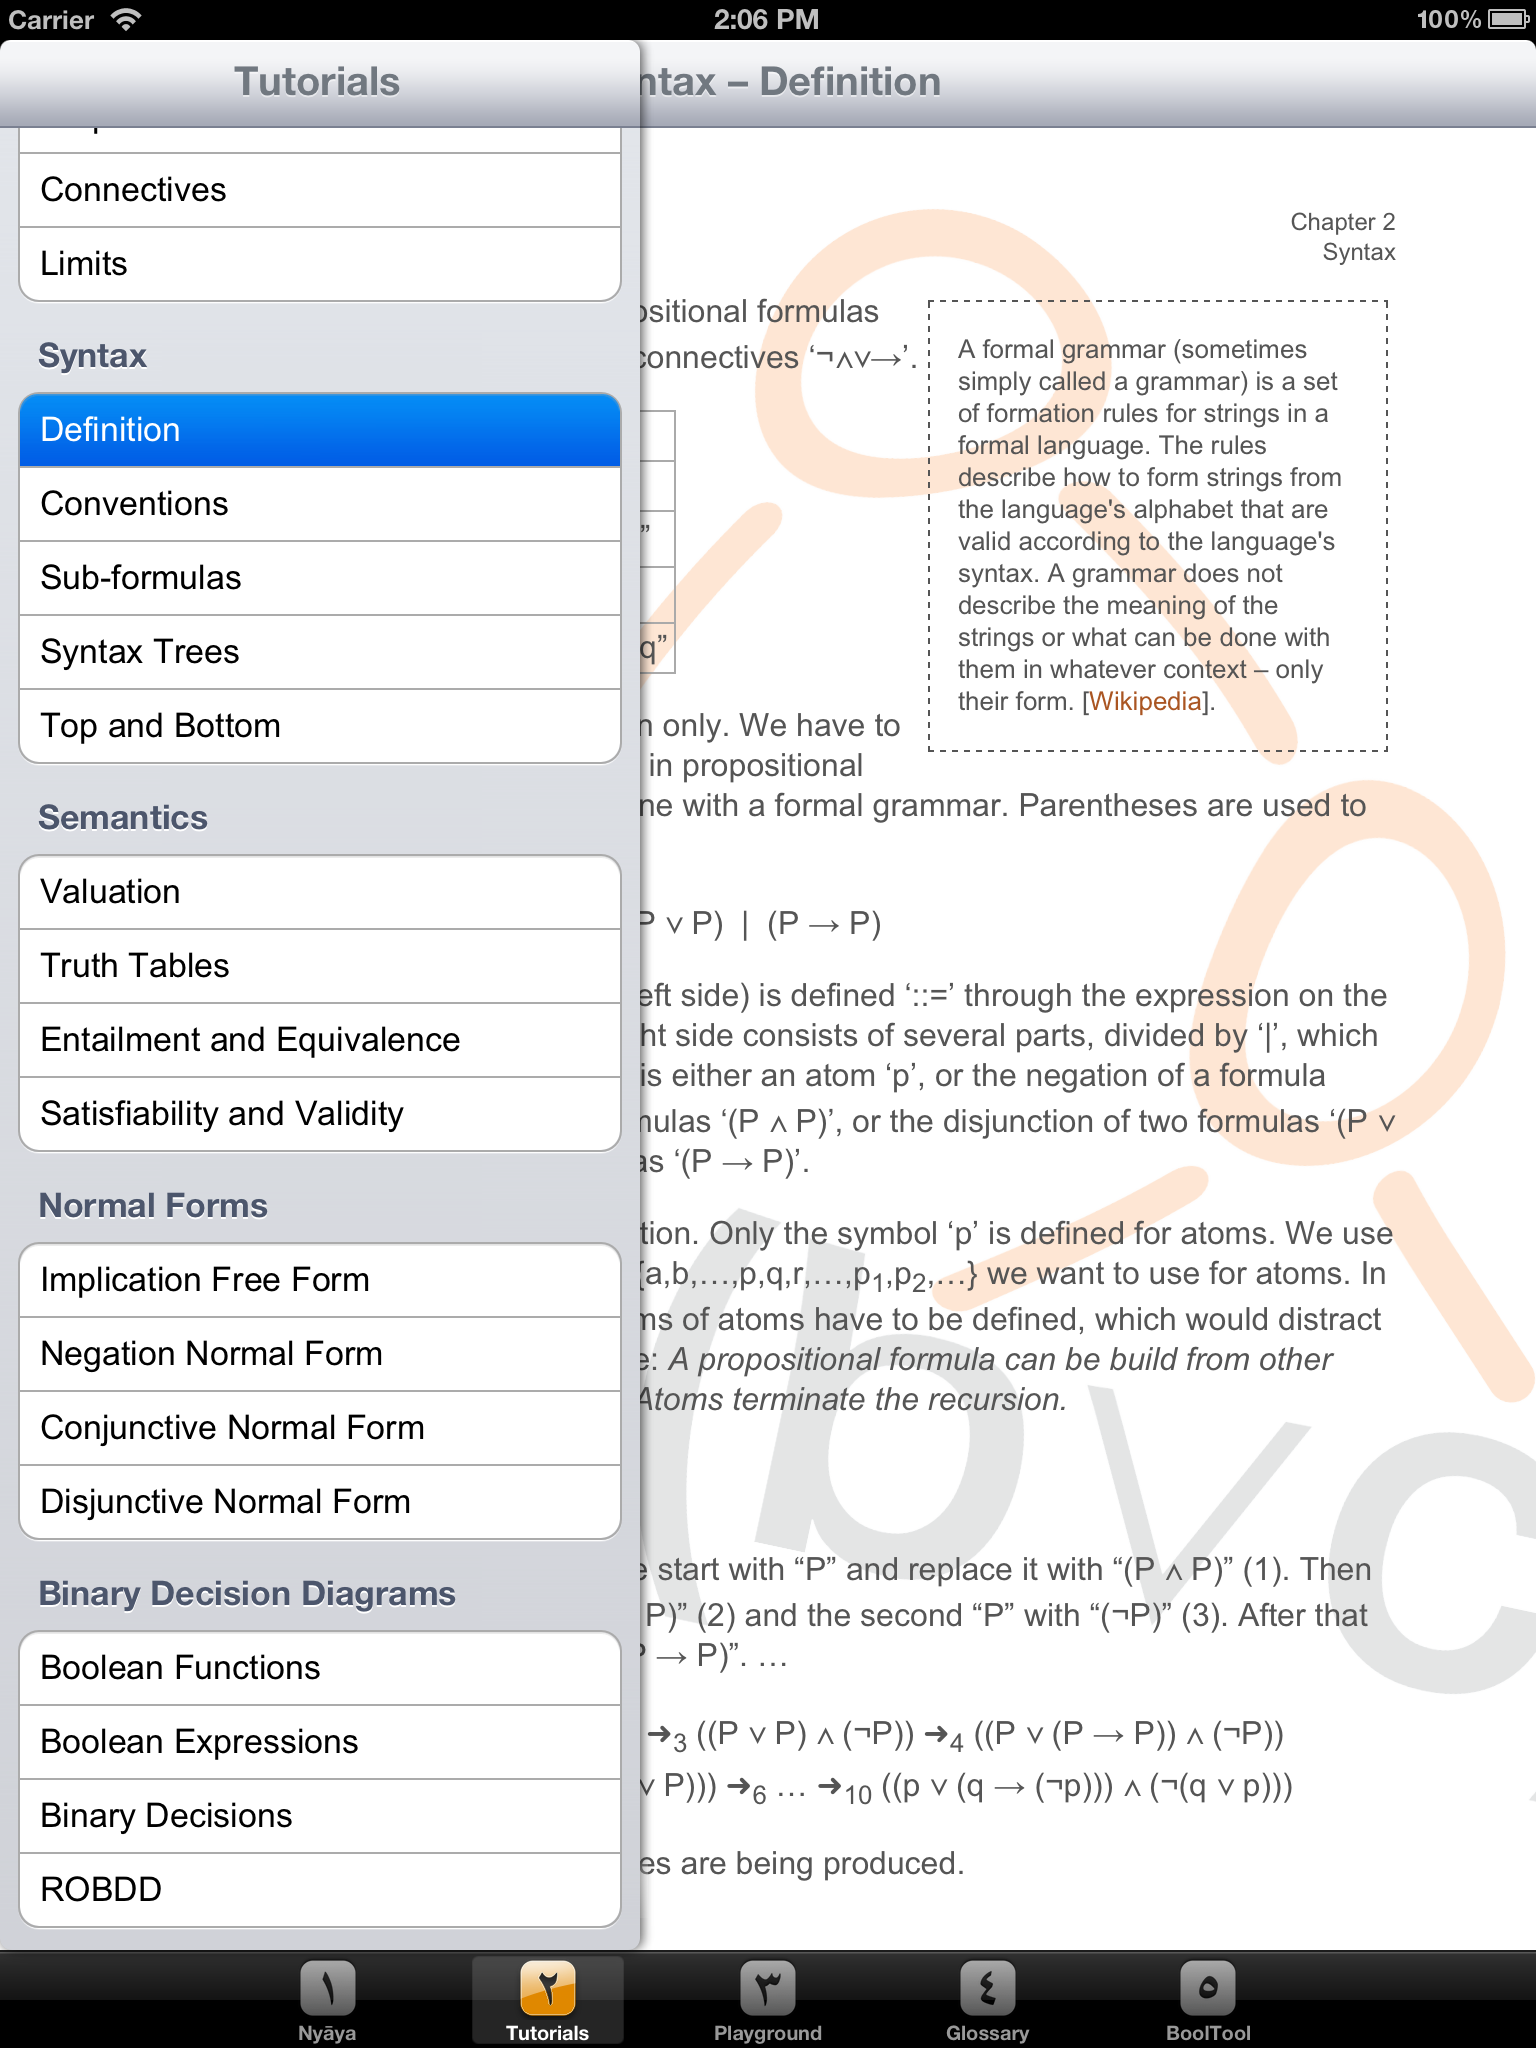
\includegraphics[width=12cm]{pics/S_Tutorials.png}
\caption{Tutorial}
\label{fig:ScreenshotTutorials}
\end{center}
\end{figure}

\begin{figure}[htbp]
\begin{center}
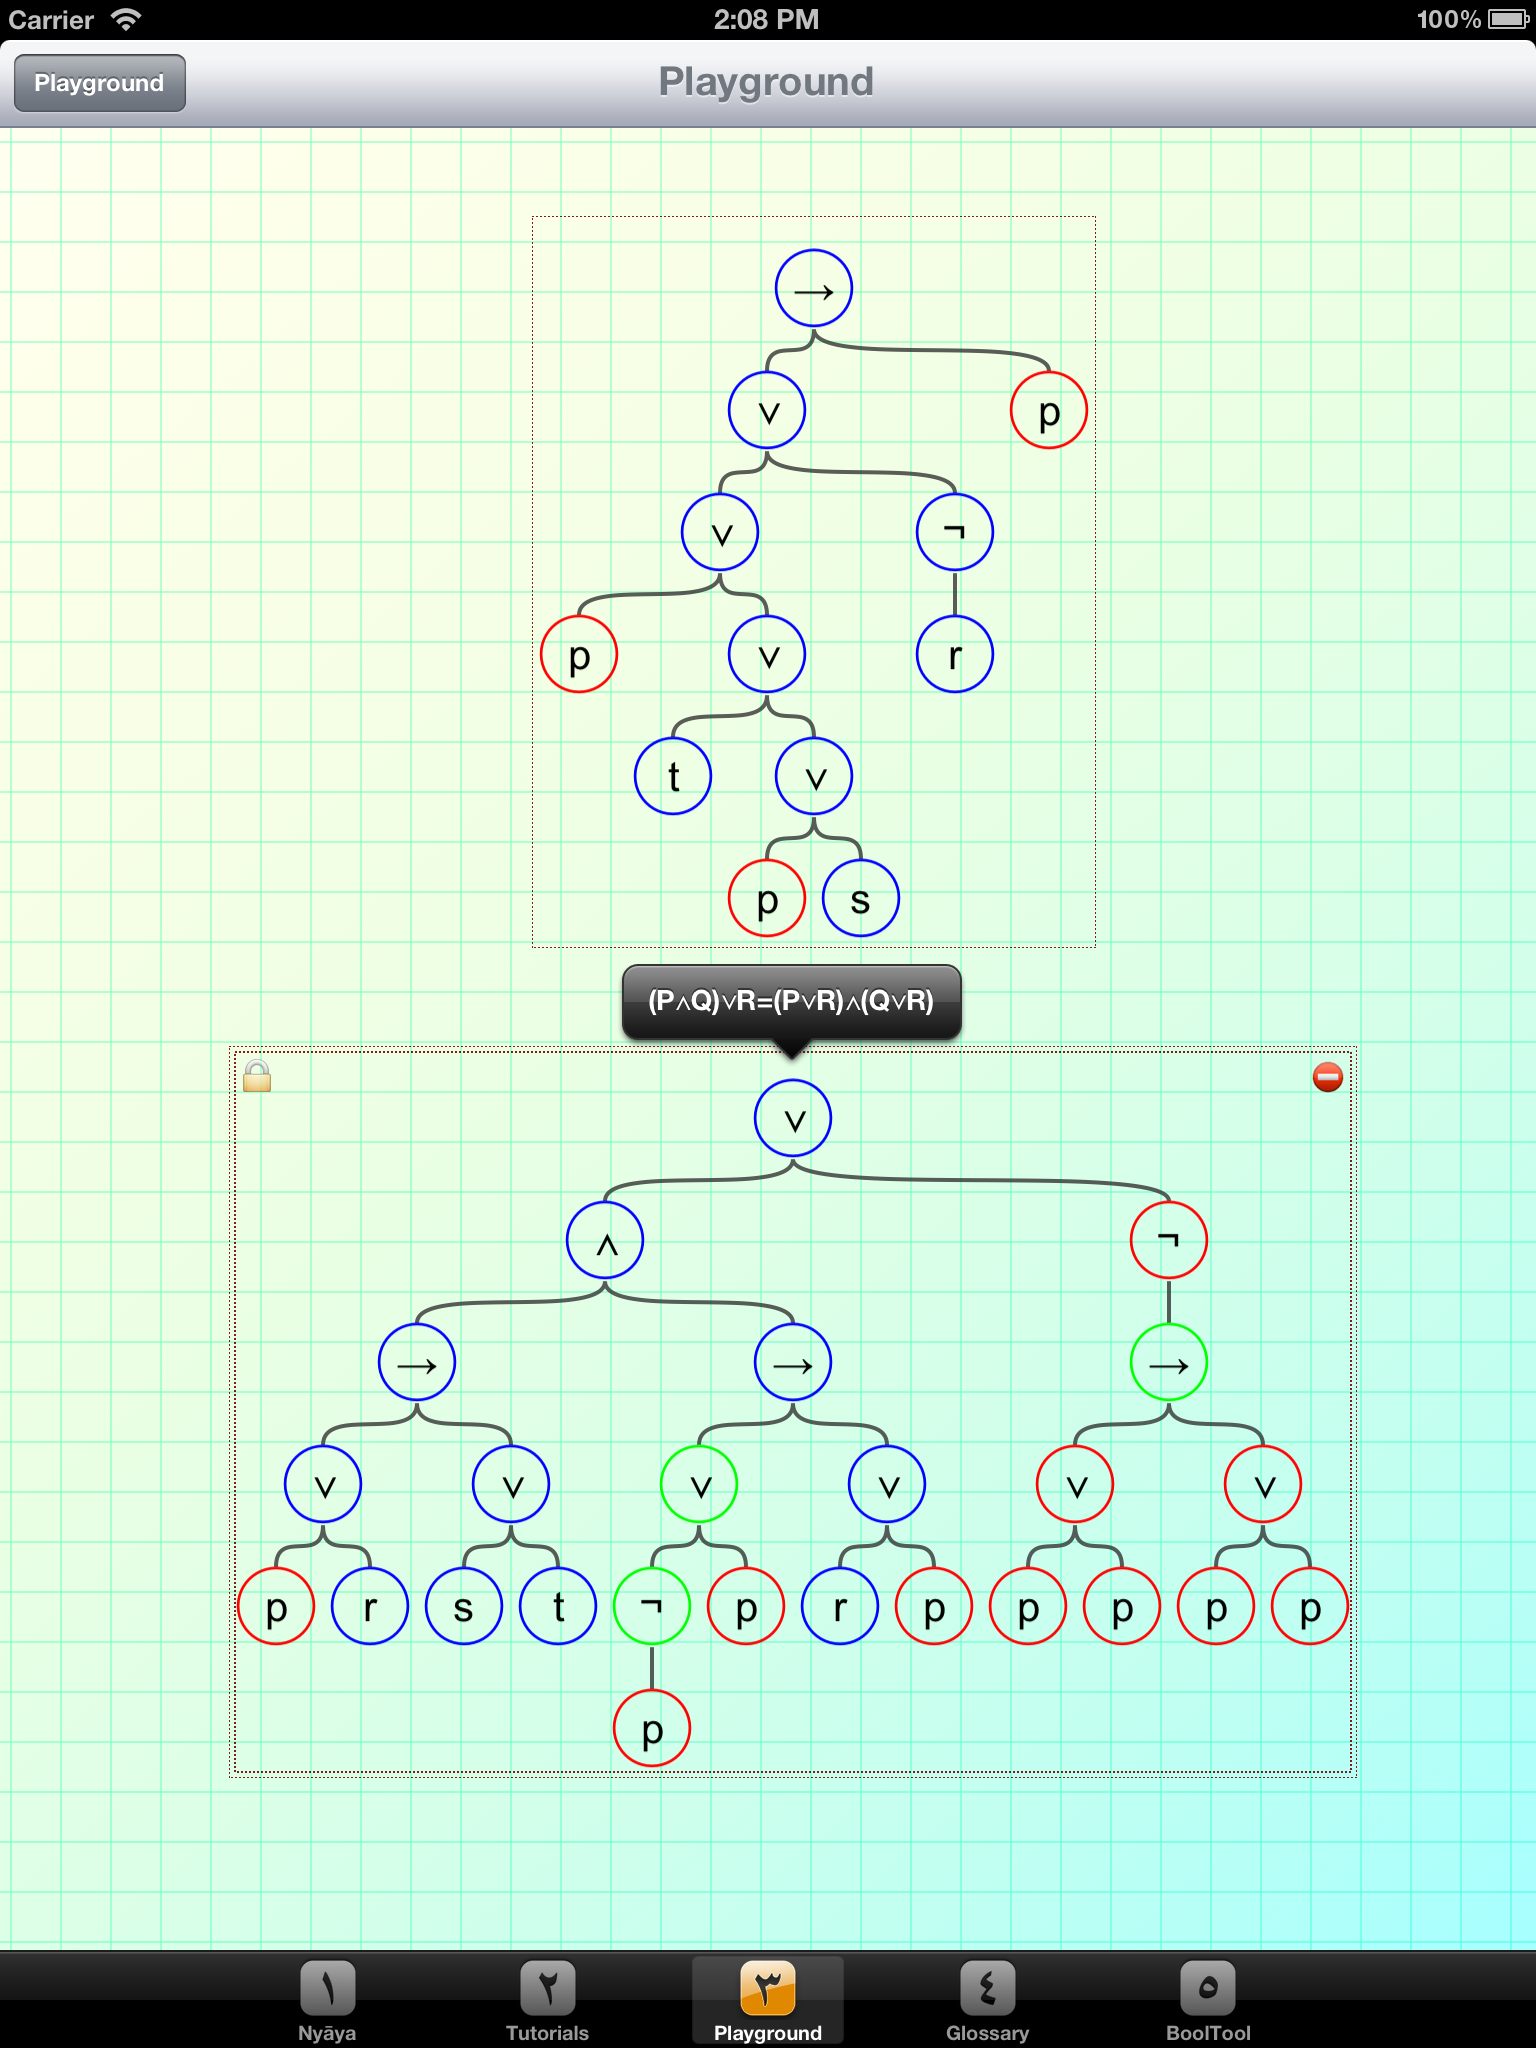
\includegraphics[width=12cm]{pics/S_Playground.png}
\caption{Playground}
\label{fig:ScreenshotPlayground}
\end{center}
\end{figure}

\begin{figure}[htbp]
\begin{center}
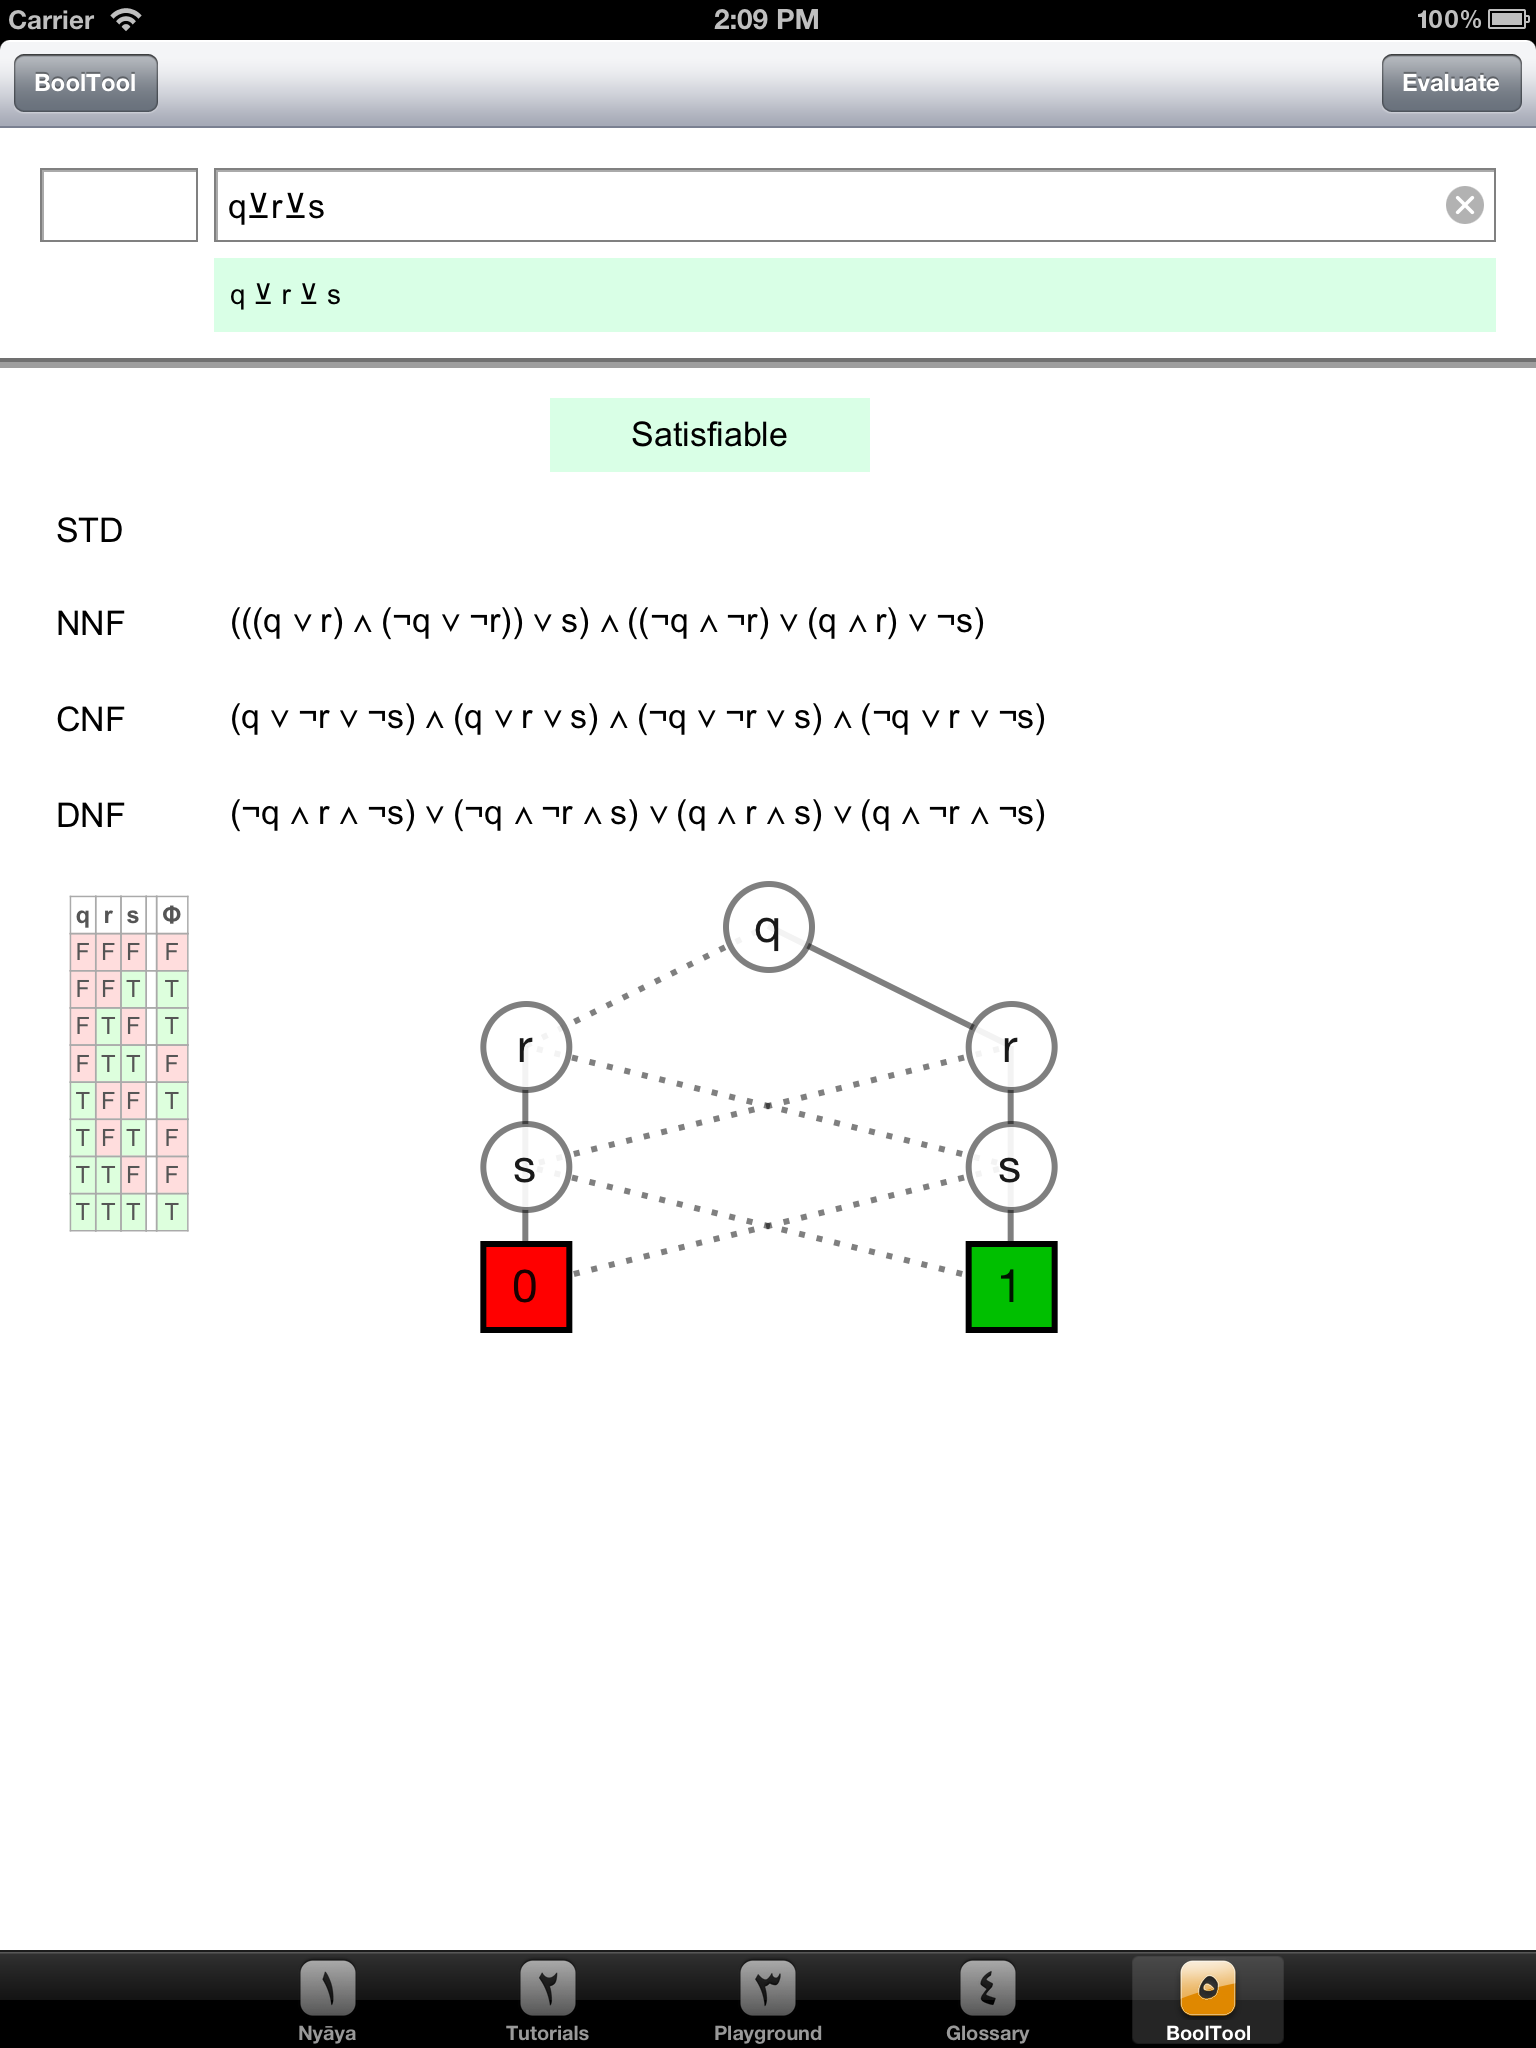
\includegraphics[width=12cm]{pics/S_BoolTool.png}
\caption{BoolTool}
\label{fig:ScrrenshotBoolTool}
\end{center}
\end{figure}






% END: appendix ------------------------------------------------------
% % !TEX encoding = UTF-8 Unicode
% ÄÖÜ ß äöü

\begin{thebibliography}{10}
% \addcontentsline{toc}{section}{Quellenverzeichnis}

\bibitem{L} Aard Middeldorp. \textit{Logic (bachelor program lecture)}. Institute of Computer Science, University of Innbruck, 2011.
\url{http://cl-informatik.uibk.ac.at/teaching/ws11/lics/content.php}

\bibitem{LICS} Michael Huth and Mark Ryan. \textit{Logic in Computer Science -- Modelling and Reasoning about Systems.} Cambridge University Press, 2nd edition, 2004 (7th printing 2011). 

\bibitem{THI} Jef Raskin. \textit{The Humane Interface -- New Directions for Designing Interactive Systems.} Addison-Wesley ACM Press, 2000 (10th printing 2008). 

\bibitem{TW} Dave Barker-Plummer, Jon Barwise, John Etchemendy. \textit{Tarski's World -- Revised And Expanded.} CSLI Publications, 2008.

\bibitem{iHIG} Apple Inc.  \textit{iOS Human Interface Guidelines} March 7th, 2011. 

\url{http://developer.apple.com/library/ios/documentation/UserExperience/Conceptual/MobileHIG/}

(\href{https://developer.apple.com/library/ios/documentation/UserExperience/Conceptual/MobileHIG/MobileHIG.pdf}
{MobileHIG.pdf} 
downloaded April 21st, 2012).

% ###############
% ## 4. Entwickler ##

%\bibitem{ADOV} Apple Inc. \textit{App Development Overview} (pdf, Stand: 12.10.2011). Internet:
%\url{http://developer.apple.com/library/mac/documentation/General/Conceptual/ApplicationDevelopmentOverview/ApplicationDevelopmentOverview.pdf} (Download: 26.11.201)

%\bibitem{TEAM} Apple Inc.: \textit{About iOS Development Team Administration}
%(web, Stand: 26.11.2011). Internet: 
%\url{http://developer.apple.com/library/ios/#documentation/ToolsLanguages/Conceptual/DevPortalGuide/Introduction/Introduction.html} (Zugriff: 26.11.2011 10:10MEZ)

%\bibitem{IOSPS} Apple Inc.: \textit{Preferences and Settings Programming Guide (iOS)} (pdf, Stand: 12.10.2011). Internet: \url{http://developer.apple.com/library/ios/documentation/Cocoa/Conceptual/UserDefaults/UserDefaults.pdf} (Download: 9.11.2011 16:13MEZ)
%
%\bibitem{MACPS} Apple Inc.: \textit{Preferences and Settings Programming Guide (Mac)} (pdf, Stand: 12.10.2011). Internet: \url{http://developer.apple.com/library/mac/documentation/Cocoa/Conceptual/UserDefaults/UserDefaults.pdf} (Download: 9.11.2011 16:16MEZ)

\bibitem{iAPG} Apple Inc.  \textit{iOS App Programming Guide.} March 7th, 2012. 

\url{http://developer.apple.com/library/ios/documentation/iPhone/Conceptual/iPhoneOSProgrammingGuide/}

(\href{http://developer.apple.com/library/ios/documentation/iPhone/Conceptual/iPhoneOSProgrammingGuide/iPhoneAppProgrammingGuide.pdf} 
{iPhoneAppProgrammingGuide.pdf}
downloaded April 21st, 2012).

\bibitem{iVPG} Apple Inc.  \textit{View Programming Guide for iOS.} March 8th, 2011. 

\url{http://developer.apple.com/library/ios/documentation/WindowsViews/Conceptual/ViewPG_iPhoneOS/}

(\href{http://developer.apple.com/library/ios/documentation/WindowsViews/Conceptual/ViewPG_iPhoneOS/ViewPG_iPhoneOS.pdf}
{ViewPG\_iPhoneOS.pdf}
downloaded April 21st, 2012).

\bibitem{cCGL} Apple Inc.  \textit{Coding Guidelines for Cocoa.} February 16th, 2012. 

\url{http://developer.apple.com/library/ios/documentation/Cocoa/Conceptual/CodingGuidelines/}

(\href{http://developer.apple.com/library/ios/documentation/Cocoa/Conceptual/CodingGuidelines/CodingGuidelines.pdf}
{CodingGuidelines.pdf}
downloaded April 21st, 2012).

\bibitem{iDPG} Apple Inc.  \textit{Drawing and Printing Guide for iOS.} September 26th, 2011. 

\url{http://developer.apple.com/library/ios/documentation/2ddrawing/conceptual/drawingprintingios/}

(\href{http://developer.apple.com/library/ios/documentation/2ddrawing/conceptual/drawingprintingios/drawingprintingios.pdf}
{drawingprintingios.pdf}
downloaded April 21st, 2012).


%\bibitem{MACOSXNEW} Apple Inc.: \textit{iCloud Storage APIs} in What's new in OS X (pdf, Stand: 1 7.2011). Internet: \url{http://developer.apple.com/library/mac/releasenotes/MacOSX/WhatsNewInOSX/WhatsNewInOSX.pdf} (Download: 25.11.2011 8:00MEZ)
%
%\bibitem{IOSDB} Apple Inc.:  \textit{Document-Based Application Programming Guide for iOS} (pdf, Stand: 12.10.2011). Internet: \url{http://developer.apple.com/library/ios/documentation/DataManagement/Conceptual/DocumentBasedAppPGiOS/DocumentBasedAppPGiOS.pdf} (Download: 9.11.2011 16:09MEZ)

\end{thebibliography}


\end{document}
